\documentclass[a4paper,11pt]{article}
%\usepackage[utf8]{inputenc}

\usepackage{amsmath, amsfonts, amsthm, amssymb}
\usepackage{tikz-cd}
\usepackage{braket}
\usepackage{cancel}
\usepackage[dvipsnames]{xcolor}
\usepackage{relsize}
\usepackage{graphicx}
\usepackage[hidelinks]{hyperref}

\renewcommand{\d}{{\mathrm{d}}}
\newcommand{\D}{{\mathcal{D}}}
\newcommand{\e}{{\mathrm{e}}}
\newcommand{\dr}[2]{\frac{\partial {#1}}{\partial{#2}}}
\newcommand{\ppi}{{\mathlarger{\mathlarger{\mathlarger{\pi}}}}}



\usepackage{geometry}
\geometry{a4paper, left=25mm, right=25mm, top=30mm, bottom=25mm}

\renewcommand{\baselinestretch}{1.2}

\begin{document}
\title{Notes de cours de\\Physique-Mathématique et Géométrie Différentielle}
\author{Cours de Frédérique Hélein - Notes de Sacha Amiel}
\date{Année 2025 - M2 Math Fonda'}
\maketitle
\tableofcontents
\newpage
\noindent\underline{Objectif}: Atteindre les théories BRST\footnote{BRST: Carlo Becchi, Alain Rouet, Raymond Stora \& Igor Tyutin} et BV\footnote{Igor Batalin \& Grigori Vilkovisky}, théories physiques dévellopées pour quantifier les théories de jauge, tout particulièrement les Yang-Mills mais aussi d'autres.

\section{Calcul des variations}
\subsection{Rappels de base de physique des particules classiques (en formalisme Lagrangien)}
\quad On considère une particule (classique) dans une variété $\mathcal{M}$ de dimension $m$; $I=]t_0,t_1[$ un intervalle réel ouvert (le temps, $t_0, t_1 \in \mathbb{R}\cup \{\pm \infty\}$); et on appel:
\begin{align*}
	``\mathrm{Lagrangien}":
		&&L:& \left\{\begin{matrix}
			I\times\mathcal{M} & \to & \mathbb{R}\\
			(t,x,v) & \mapsto & L(t,x,v)
		\end{matrix}\right.\\
	``\mathrm{Action}":  && \mathcal{A} :& \left\{\begin{matrix}
			\mathcal{C}^1(I,\mathcal{M}) & \to & \mathbb{R}&\\
			\gamma & \mapsto & \mathcal{A}[\gamma]&:=\int_I L\big(t,\gamma(t),\dot \gamma(t)\big)
		\end{matrix}\right.
\end{align*}
où $L$ est au moins $\mathcal{C}^1$ en $x$ et $\mathcal{C}^2$ en $v$, et où
\begin{equation*}\begin{split}
\delta\mathcal{A}_\gamma[\delta\gamma]
&=\int_I \dr{L}{x^i}(t,\gamma,\dot \gamma)\delta\gamma^i + \dr{L}{v^i}(t,\gamma, \dot \gamma)\frac{\d \delta \gamma^i}{\d t}\\
&=\int_I \frac{\d}{\d t}\left(\dr{L}{v^i}(t,\gamma,\dot \gamma)\delta\gamma^i \right)+ \left(\dr{L}{x^i}(t,\gamma, \dot \gamma) - \frac{\d}{\d t}\dr{L}{v^i}\right)\delta \gamma^i
\end{split}\end{equation*}

\underline{Principe de Maupertuis} (généralisé): On obtient les trajectoires d'une physique classique régie par $L$ en se restreignant à l'ensemble des chemins $\gamma$ tels que $\forall \delta \gamma \quad \delta\mathcal{A}_\gamma[\delta_\gamma]=0$. i.e. ce sont les chemins qui extremisent localement l'action (hors cas physique, on parlera donc simplement de ``points critiques").\\ \\
D'où on dérive le \underline{principe d'Hamiltion}: 
$\forall \delta\gamma \; \mathrm{t}.\mathrm{q}.\; \delta\gamma(t_0)=\delta\gamma(t_1)=0$
\begin{equation*}
\;_{(\mathrm{Maup})} \; \delta\mathcal{A}_\gamma[\delta\gamma] = 0 \quad \quad \iff \quad \quad \boxed{\frac{\d}{\d t}\left(\dr{L}{v_i}(t,\gamma,\dot\gamma)\right) = \dr{L}{x^i}(t,\gamma,\dot\gamma)}_{\quad(\mathrm{E}.\scalebox{0.75}[1.0]{-}\mathrm{L}.)}
\end{equation*}
où l'équation à droite est appelée ``equations d'\underline{Euler-Lagrange}" (E.-L.) (pour une physique de particules). (Existe aussi en version théorie de champs, cf plus tard).

\subsection{1$^\mathrm{er}$ théorème de Noether, symétries et conservation (cas des particules)}
Première difficulté: qu'est-ce qu'une symétrie? Il s'agit, grossièrement d'une action d'un groupe de Lie. (Enfin, d'une algèbre de Lie plutôt...)\\
Version simple:\\
\begin{minipage}{.5\textwidth}
\centering
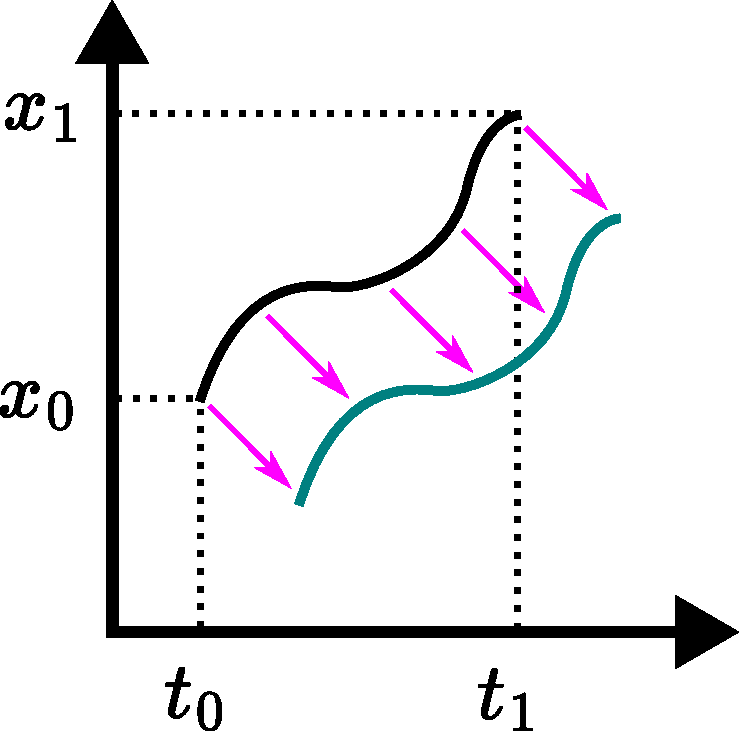
\includegraphics[width=.5\textwidth]{Drawings/Draw_1.pdf}
\end{minipage}
\begin{minipage}{.5\textwidth}
\centering
$$X = X^0(t,x)\frac{\partial}{\partial t} + X^i(t,x) \frac{\partial}{\partial x^i}$$
$$T:=X^0$$
\end{minipage}

\noindent On note $\Delta_X\subset \mathbb{R}\times(I\times\mathcal{M})$ maximal sur lequel le flot est défini.
\begin{equation*}
	\Phi_X : \left\{\begin{matrix}
	\Delta_X & \to & I\times\mathcal{M} &\\
	(\epsilon,t,x) & \mapsto & \Phi_X(\epsilon,t,x) &=\e^{\epsilon X}(t,x)
	\end{matrix}\right.
\end{equation*}
i.e. $\frac{\partial \Phi}{\partial \epsilon}(\epsilon, t, x) = X(\Phi_X(\epsilon, t, x))$ et $\Phi_X(0,t,x)=(t,x)$
\\
en coord loc, ça donne: $\e^{\epsilon X}(t,x)=\left(\quad t+\epsilon T(t,x),\quad x^i+\epsilon X^i(t,x)\quad \right) + o(\epsilon)$
\\
Action sur $\mathcal{C}^1(I',\mathcal{M})$ où $I'$ est un intervalle compacte de $I$:
\begin{align*}
\gamma &\mapsto \gamma_\epsilon\\
[t_0,t_1] &\mapsto[t_0(\epsilon),t_1(\epsilon)]=[t_0+\epsilon T(t_0,x_0),t_1+\epsilon T(t_1,x_1)]\quad \mathrm{modulo}\;\epsilon
\end{align*}
\begin{align*}
\forall i \in [\![1,n]\!] \quad \gamma^i_{\epsilon}(\Phi_X^0(\epsilon,t,x) &= \Phi_X^i(\epsilon,t,\gamma(t))\\
\gamma_\epsilon &= \gamma + \epsilon\delta\gamma + o(\epsilon)
\end{align*}
\begin{align*}
(\gamma^i+\epsilon\delta\gamma^i)(t+\epsilon T(t,\gamma)) = \gamma^i + \epsilon X^i(t,\gamma) + o(\epsilon)
&\iff \frac{\d \gamma^i}{\d t}T + \delta\gamma^i = X^i\\
&\iff \boxed{\delta \gamma^i = X^i(t,\gamma) - T(t,\gamma)\dot\gamma^i}
\end{align*}
$$X \; \mathrm{symetrie}\;\mathrm{de}\;L \overset{(\mathrm{def})}{\iff} \forall [t_0,t_1]\subset I \quad \int_{t_0(\epsilon)}^{t_1(\epsilon)} L(t,\gamma_\epsilon, \dot\gamma_\epsilon)\d t = \int_{t_0}^{t_1} L(t,\gamma,\dot\gamma)\d t + (\epsilon)$$
\underline{Théorème 1}: Si $X$ est une symétrie et si $\gamma$ est un point critique alors
$$Q_X(t) := \dr{L}{v^i}(t,\gamma,\dot\gamma)X^i(t,\gamma) - \left(\dr{L}{v^i}(t,\gamma,\dot\gamma)\dot\gamma^i - L(t,\gamma,\dot\gamma)\right)T(t,\gamma)$$
est conservé (i.e. $\frac{\d Q}{\d t}=0$).\\
\\
\underline{Remarque}: $Q_X = \dr{L}{v^i} + LT$\\ \\
Preuve du théorème:
$\forall \gamma \in \mathcal{C}^1(I,\mathcal{M})$\\
\begin{align*}
1) \;\mathrm{hypothese}\;\mathrm{de}\;\mathrm{symetrie}\;
&\iff \int_{t_0}^{t_1} L(t,\gamma_\epsilon,\dot\gamma_\epsilon) = \int_{t_0}^{t_1}L(t,\gamma,\dot\gamma) + \epsilon [LT]_{t_0}^{t_1} + \int_{t_0}^{t_1} \left(\dr{L}{x^i}\delta \gamma^i + \dr{L}{v^i}\delta\dot\gamma^i\right) +o(\epsilon)\\
&\iff \int_{t_0}^{t_1} \delta_X L(t,\gamma,\dot\gamma) \d t:=\int_{t_0}^{t_1} \left(\dr{L}{x^i}\delta \gamma^i + \dr{L}{v_i}\delta\dot \gamma^i + \frac{\d (LT)}{\d t}\right)\d t =0
\end{align*}
où $\delta_X L : I\times T\mathcal{M} \to \mathbb{R}$. 
Bref, ``symétrie $\implies \delta_X L = 0$".\\
\\
\underline{Exo}: construire $\delta_X L$ et montrer que ça marche...\\
\\
2) Montrons que $Q$ constant si (et seulement si) $\gamma$ est un point critique.
$$\frac{\delta L}{\delta \gamma^i} := \dr{L}{x^i}(t,\gamma,\dot\gamma) - \frac{\d}{\d t}(\dr{L}{v^i}(t,\gamma,\dot\gamma))$$
D'où EL $\iff \frac{\delta L}{\delta \gamma^i}=0$
\begin{align*}
\dr{L}{x^i}&= \frac{\delta L}{\delta \gamma^i} + \frac{\d}{\d t}(\dr{L}{v^i})\\
\frac{\d Q_X}{\d t}
&= \frac{\d}{\d t} (\dr{L}{v^i}\delta \gamma^i + LT)\\
&= \frac{\d}{\d t} (\dr{L}{v^i})\delta \gamma^i + \dr{L}{v^i} \delta\dot\gamma^i+\frac{\d}{\d t}(LT)\\
&= \dr{L}{x^i} \delta^i+\dr{L}{v^i}\delta \dot \gamma + \frac{\d (LT)}{\d t} - \!\!\!\!\!\!\!\!\!\!\!\!\!\!
\underset{\quad\quad\quad=0\;\mathrm{par}\;(\mathrm{E}.\scalebox{0.75}[1.0]{-}\mathrm{L}.)}{\cancel{\frac{\delta L}{\delta \gamma^i}\delta \gamma^i}}\\
&=0 \quad \mathrm{par} \; \mathrm{symetrie}
\end{align*}
\\
\underline{Variante}: Si $\exists f:I\times\mathcal{M}\to \mathbb{R}$ t.q. $\delta_X L(t,\gamma,\dot\gamma) = \frac{\partial f}{\partial t}(t,x) + v^i \frac{\partial f}{\partial x^i}(t,x)$ ``symétrie modulo un terme exacte" (def) alors la quantité conservée est $(Q_X -f)$.\\

Même si on va aller plus loin dans les théorèmes de Noether plus tard, une bonne référence (historique) est \emph{Les Théorèmes de Noether: Invariance et lois de conservation au XXe siècle} par  Yvette Kosmann-Schwarzbach, éditions de l'école Polytechnique, ISBN: 978-2730211383.


\subsection{Formalisme Hamiltonien}
L'idée est de faire un changement de variable de $T\mathcal{M}$ vers $T^*\mathcal{M}$... Commençons par définir une variété symplectique.
\\
\underline{Définition}: (variété symplectique)\\
Une var symplectique $\mathcal{M}$ est une variété munie d'une 2-forme $\omega$, $\omega \in \Omega^2(\mathcal{M})$ telle que:
\begin{itemize}
\item $\omega$ non dégénérée i.e. $\forall \xi\in T\mathcal{M}, \quad \quad \xi \lrcorner \omega = 0 \quad \implies \quad \xi =0$\\
$\xi \lrcorner \omega:= \omega(\xi,\cdot)$ (également noté, $\iota_\xi \omega$ dans d'autres ressources)
\item $\d \omega = 0$\quad\quad ``forme fermée"
\end{itemize}

Dans des coordonnées locales, $\omega = \sum_{1\leq a_1 < a_2\leq n} \omega_{a_1a_2} \d x^{a_1} \wedge \d x^{a_2}$, et les hypothèses reviennent à dire que le rang de la matrice $(w_{a_1a_2})$ est maximal, d'où dim$\mathcal{M}$ paire.\\
\\
\underline{Théorème de Darboux}:\\
Dans toute variété symplectique, tout point admet une carte (et un jeu de coordonnées $(p_i)\!\!\smile\!\!(q^i)$ sur cet ouvert) dans laquelle $\omega = \d p_i\wedge\d q^i$.\\
\\
Constructions ultra classiques de var symplectiques:\\
a) $\mathbb{R}^{2n}=\mathbb{R}^n\times\mathbb{R}^n$, on peut donc définir $\omega$ comme dans le théorème de Darboux sur tout $\mathbb{R}^{2n}$.
\\
b) Soit $\mathcal{M}$ une variété de dimension $n$, 
\begin{equation*}
\exists!\; \pi : \left\{\begin{matrix}
(T^*\mathcal{M}) & \to & \mathcal{M} \\
(q,p) & \mapsto & q
\end{matrix}\right.
\end{equation*}
Soit ce $\pi$ et soit $\theta \in \Omega^1 (T^*\mathcal{M})$ tel que,
$$\forall \xi \in T_{(p,q)}(T^*\mathcal{M}), \quad \theta_{(q,p)}(\xi) = \langle \underset{\in T_q^*\mathcal{M}}{p,} \underset{\in T_q\mathcal{M}}{\d \pi_{(q,p)} \xi} \rangle$$

En coordonnées locales, $(q^i)$ sur $\mathcal{M}$ et $(p_i)$ sur $T_q^*\mathcal{M}$ avec $p := p_i \d q^i$, on obtient $\theta = p_i \d \left(q^i\circ \pi\right)$ où $(p_i)\!\!\smile\!\!(q^i)$ sont des coordonnées locales sur $T^*\mathcal{M}$. On notera tout simplement $\theta = p_i\d q^i$ avec $\theta \in \Omega^1(T^*\mathcal{M})$
ce qui est un abus de notation conséquent (notamment puisque rentrant violemment en conflit avec la définition de $p$). Bref, il faut ouvrir l'œil au contexte.\\
\\
Il suffit alors de prendre $\omega := \d \theta$ forme symplectique, pour avoir $(T^*\mathcal{M},\omega)$ une variété symplectique.

\noindent \underline{Lien entre Lagrangien et géométrie symplectique} (eq° de Hamilton)\\
L'objectif est d'effectuer une transformation de la forme:
\begin{equation*}
L: \left\{ \begin{matrix}
\mathbb{R}\times T \mathcal{M} & \to & \mathbb{R}\\
(t,x,v) & \to & L(t,x,v)
\end{matrix}\right.
\quad \leftrightsquigarrow \quad H:\left\{\begin{matrix}
\mathbb{R}\times T^* \mathcal{M} & \to & \mathbb{R}\\
(t,q,p) & \to & H(t,q,p)
\end{matrix}\right.
\end{equation*}

Si $(\d q^i)$ est une base de $T_q^*\mathcal{M}$, $p\in T^*_q\mathcal{M} \implies p=p_i\d q^i$, d'où $(p_i, q^i)$ est un système de coordonnées sur $T^*\mathcal{M}$; enfin, en fait c'est $q^i\circ \pi$ à la place de $q^i$ mais bon, c'est l'abus de notation de tout à l'heure. On pose:
$$\theta = p_i\d q^i$$
\underline{Transformation de Legendre}:
$$\forall (t,q) \in \mathbb{R}\times\mathcal{M}\quad\quad \d \left(L_{|\{t\}\times T_q\mathcal{M}}\right) =: \dr{L}{v}(t,q,v)$$
en coordonnés locales, $v=v^i\frac{\partial}{\partial q^i} \in T_q\mathcal{M}$
$$\dr{L}{v} = \dr{L}{v^i} \d v^i$$
Hypothèse de Legendre: 
\begin{equation*}
\mathbb{L}: \left\{\begin{matrix}
\mathbb{R}\times T\mathcal{M} & \to & \mathbb{R}\times T^*\mathcal{M}\\
(t,q,v) & \mapsto & (t,q, \dr{L}{v}(t,q,v))
\end{matrix}\right. \quad \mathrm{est}\; \mathrm{un}\; \mathrm{diffeo}
\end{equation*}
Exemple: $L = \frac{m |v|^2}{2} - V(q)$\\
\\
\underline{Définition}: (Hamiltonien)
\begin{align*}
H : \mathbb{R}\times T^*\mathcal{M} &\to \mathbb{R}\\
(H\circ\mathbb{L})(t,q,v) &= \dr{L}{v^i}(t,q,v) v^i - L(t,q,v)\\
\iff (\mathrm{implicit})\quad  \mathbb{L}^{-1}&: (t,q,p)\to (t,q,v(t,q,p))
\end{align*}
$$\dr{L}{v^i}(t,q,v(t,q,p)) =: p_i $$
$$H(t,q,p) = p_i v^i(t,q,p) - L(t,q,v(t,q,p))$$

\subsection{Retours sur Noether}
$T\frac{\partial}{\partial t} + X^i \frac{\partial}{\partial x^i}$ sur $\mathbb{R}\times\mathcal{M}$ est une symétrie de $L$.

$\implies Q = \dr{L}{v^i}(t,\gamma, \dot\gamma)X^i(t,\gamma) - (\dr{L}{v^i}\dot\gamma^i - L(t,\gamma,\dot\gamma))$ est conservé si $\gamma$ est solution.

$$Q = \underset{``\mathrm{moment}"}{(p_i \circ \mathbb{L})}X^i - \underset{``\mathrm{energie}"}{(H\circ\mathbb{L})}T$$
\begin{align*}
\d H &= v^i \d p_i + \cancel{p_i\d v^i} - \dr{L}{t}(t,q,v) \d t - \dr{L}{q_i}\d q^i - \cancel{\dr{L}{v^i}(t,q,v(t,q,p) \d(v^i)}\\
&= v^i\d p_i - (\dr{L}{t}\circ \mathbb{L}^{-1})\d t - (\dr{L}{q^i}\circ \mathbb{L}^{-1}) \d q^i
\end{align*}
D'où 
\begin{align*}
	\dr{H}{t} &= -\dr{L}{t}\circ \mathbb{L}\\
	\dr{H}{q^i} &= - \dr{L}{x^i} \circ \mathbb{L}\\
	\dr{H}{p_i} &= v^i
\end{align*}
d'où $\forall \gamma:\mathbb{R} \to \mathcal{M}$
$$\pi = \dr{L}{v}(t,\gamma,\frac{\d \gamma}{\d t})$$\\

\noindent \underline{Lemme}: (transition Lagrangien-Hamiltonien)
\begin{equation*}
\frac{\d}{\d t} (\dr L{v^i} (t,\gamma, \dot \gamma)) = \dr L{q_i} (t,\gamma,\dot\gamma)\quad (\mathrm{EL}) \quad \iff \quad
\left\{\begin{split} \frac{\d \gamma^i}{\d t}&=\dr{H}{p_i}(t,\gamma,\pi) \quad (\mathrm{Hq})\\
\frac{\d \pi_i}{\d t}&=-\dr{H}{q^i}(t,\gamma,\pi) \quad (\mathrm{Hp})\end{split}\right.
\quad\quad\quad\quad\quad\quad\quad\quad\quad\quad\quad\quad\quad\quad\quad\quad\quad\quad\quad\quad\quad\quad\quad\quad\quad\quad\quad\quad\quad\quad\quad
\end{equation*}
Preuve:
$$Hq \iff (t\gamma,\pi) = \mathbb{L}(t,\gamma,\dot\gamma)$$
$$\dr{H}{p_i}(t,\gamma,\pi)=v^i(t,\gamma,\pi)=\frac{\d \gamma^i}{\d t}$$
par def de $v$.\\
Alors, $\pi_i = \dr{L}{v_i}(t,\gamma,\dot\gamma)$
$$\frac{\d \pi}{\d t} = \frac{\d}{d t}(\dr{L}{v_i}) \overset{(\mathrm{E.L.})}= \dr{L}{x^i} = -\dr{H}{q^i}$$
Notation:
\begin{align*}
\frac{\d q^i}{\d t} &= \;\;\,\dr H{p_i}\;\\
\frac{\d p_i}{\d t} &= -\dr H{q^i}
\end{align*}

\subsection{Formulation Géométrique}
$t\mapsto (\gamma(t), \pi(t)) \in \mathcal{C}^1(\mathbb{R},T^*\mathcal{M})$ est solution de Hamiltion
$$\iff \frac{\d}{\d t}(\gamma^i, \pi_i) = (\dr H{p_i},-\dr H{q^i})(\gamma,\pi)$$
champ de vecteurs \color{red} non-autonome (i.e. indépendant de $t$) \color{black} tangent à $T^*\mathcal{M}$.
$$X_H = \dr H{p_i} \dr{}{q^i}-\dr H{q^i}\dr{}{p_i}$$
$$\omega = \d p_i \wedge \d q^i$$
\begin{align*}
X_H \lrcorner \omega
&= \left(\dr H{p_i} \dr{}{q^i}-\dr H{q^i}\dr{}{p_i}\right) \lrcorner \d p_j\d q^j\\
&= \dr H {p_i} (-\delta^{ij} \d p_j) - \dr H {q^i}(\delta_{ij}\d q^j)\\
&= - \left(\dr H {p_i} \d p_i + \dr H {q^i} \d q^i\right)\\
&=\dr H t - \d H
\end{align*}
bref:
$$\boxed{X_H \lrcorner \omega + \d H = \dr H t \d t}$$
Artifice: $T^*(\mathbb{R}\times\mathcal{M}) \supset (\mathbb{R}\times\{0\})\times T^*\mathcal{M}\approx\mathbb{R}\times T^*\mathcal{M} $
\\
On pose alors $q^0 = t$ et sur $T^*(\mathbb{R}\times\mathcal{M})$ on étends $\Tilde \omega:= \d p_0 \wedge \d t + \d p_i \wedge \d q^i$ d'où
$$X_{\Tilde H} \lrcorner \Tilde \omega + \d \Tilde H=0$$
et donc on s'intéresse uniquement à l'hyper-surface $p^0 = H$.

\section{Théorèmes de Noether généraux}
\subsection{Théorème 1}
Lagrangien d'ordre quelconque $r$, i.e. $L(x, \dot x, \ddot x, \dot{\ddot x}\;...\; x^{(r)})$. On travaille sur des champs $u:U\to\mathcal{M}$ où $U=\mathbb{R}$ dans le cas particules, mais sinon peut-être n'importe quoi (ligne d'univers d'une particule dans l'espace-temps, champ classique, ou des produits de ça...).
\\
\underline{Définition}: (Jets)\\
Si $\mathcal{M}$ est varr de dim $k$ et $U$ est un ouvert de $\mathbb{R}^n$, 
$$\mathfrak{j}^r u (x) := \Big(x, u(x), \partial u(x), \partial^2 u(x), \,...\, \partial^r u (x)\Big)$$
où $\partial^i := \dr{}{^{\mu_1}...\partial^{\mu_i}} =: \partial_{\mu_1...\mu_i}$. 
Cas général pour des variétés quelconques:

\begin{align*}
	\mathfrak{j}^0(U,\mathcal{M}) &= U\times\mathcal{M}\\
	\mathfrak{j}^1(U,\mathcal{M}) &= \Big\{(x,y,E), \quad (x,y)\in U\times\mathcal{M}, E \;\mathrm{sev}\;\mathrm{de}\; T_{(x,y)}(U\times\mathcal{M})\\&\quad \quad| \quad \mathrm{dim}E=\mathrm{dim}U\\
	&\quad\quad\quad\;\d (\pi_{U\times\mathcal{M}\to U})_{(x,y)}: T_{(x,y)}(U\times\mathcal{M})\to T_x\mathcal{M}
	\\&\quad\quad\quad\; \d (\pi_{U\times\mathcal{M}\to U})_{x,y)}|_E : E\to T_x\mathcal{U}\quad\quad\quad\quad\quad\quad\quad\quad\quad\Big\}\\
	\mathfrak{j}^r(U,\mathcal{M}) &= \mathfrak{j}^1(U, j^{r-1}(U,\mathcal{M}))
\end{align*}
Système de coordonnées locales sur les jets:
$$v^i_{\mu_1...\mu_j} \quad\quad \mathrm{t}.\mathrm{q}. \quad\quad v^i_{\mu_1...\mu_j}(j^ru(x))=\dr{u^i}{x^{\mu_1}...\partial x^{\mu_j}}$$
Lagrangien général d'ordre $r$ sur ``$U\to\mathcal{M}$":
$$L : j^r(U,\mathcal{M}) \to \mathbb{R}$$
$$\mathcal{L}[u] = \int_{U} L(j^r u(x))\d^n x$$

Symétrie infinitésimale $u\mapsto u+\epsilon\delta u + o(\epsilon)$ infinitésimales, générés par un champ de vecteurs $Z$ sur $U\times\mathcal{M}$. Ou plutôt, pour être précis, un champ $Z:j^r(u)\to T(U\times\mathcal{M})$.
$$Z = X^\mu \partial_\mu + Y^i  \partial_i$$
$$\delta u^i = Y^i - \dr{u^i}{x^\mu}X^\mu$$
\underline{Théorème de Noether 1}: (Forme la plus générale)

Si $L$ est invariant par $X^\mu\partial_\mu + Y^i\partial_i$ et si $u$ est un point critique de $\mathcal{L}$ alors il lui correspond $J^\mu\partial_\mu$ définit sur $U$ tel que $\dr {J^\mu}{x^\mu}=0$\\
\\
Ex: $u: \mathbb{R}^n \to \mathbb{R}$ \quad\quad $\Omega\subset \mathbb{R}^n$
\quad \quad $\mathcal{L}[u]=\int_{\Omega} \frac{|\nabla u|^2}2 \d x$ (action de Dirichlet)\\
$\mathcal{L}[u+\epsilon\varphi] = \int_\omega \frac{|\nabla u|^2}2 + \epsilon \langle\nabla u, \nabla \varphi\rangle + \epsilon^2 \frac{|\nabla \varphi|^2}2$
 ($\varphi$ supposé à support compacte.)
\begin{align*}
\delta \mathcal{L}_u[\varphi] &= \int_\Omega \langle\nabla u, \nabla \varphi\rangle \d x\\
&= \int_\Omega \big(\mathrm{div}(\varphi\nabla u) - \varphi \Delta u\big) \d x\\
&=- \int \varphi \Delta u
\end{align*}
Symétrie par translation $u \mapsto u\circ \tau_\epsilon =: u_\epsilon$; $\tau_\epsilon (x) := x-\epsilon v$.\\
$u_\epsilon(x) = u(x-\epsilon v) \approx u(x) - \epsilon v^i \dr u {x^i}(x) + o(\epsilon)$\\
$\delta u = - v^i \dr u {x^i}$\\
Noether: Si $\delta u = 0$, 
$$\dr L {v_\mu} (x,u,\d u) \dr u {x^\nu} - (L(x,u, \d x) \delta_\mu^\nu) v^\mu = J^\nu$$
alors $\dr{J^\nu}{x^\nu} = 0$\\
(le prof est pas totalement sûr de la formule pour $J$, voir la démo qui suit)\\
\underline{Cas particulier}:
$r=1$, i.e. $L(x,u,\partial u)$, $X^\mu (x,u), Y^i(x,u)$
$$J^\mu = \dr L {v^i} (x,u,\partial u) Y^i - \left(\dr L {v^i_\mu} \dr{u^i}{x^\nu} - L \delta_\nu^\mu\right) X^\nu$$
et EL $\implies \dr{J^\mu}{x^\mu}=0$\\
\underline{Démonstration}: (cas général)\\
$X^\mu \partial_\mu + Y^i \partial_i$ agissant sur $(U,u)$.\\
$U\mapsto U_\epsilon=\varphi_\epsilon(U)$.\\
$\varphi_\epsilon := x + \epsilon X + o(\epsilon)$.
$u\mapsto u_\epsilon = u + \epsilon \delta u + o(\epsilon)$.
$$\delta u^i := Y^i - \dr{u^i}{x^\mu}X^\mu$$
Symétrie $\overset{\mathrm{def}}{\iff} \quad \forall U \forall u \quad \mathcal{L}_{U_\epsilon}[e_\epsilon] = \mathcal{L} + o(\epsilon)$\\
Petit lemme de calcul ($m$ multi-indice):
$$0 = \int_U \left[\sum_{|m|<r}\dr L{v^i_m}\big(\mathfrak{j}^r(u)\big)\dr{^m\delta u^i}{x^m}+\dr{}{x^\mu}\big(L(\mathfrak{j}^r(u)X^\mu\big) \right] \d^n x$$
autre petit lemme:\\
$\rho(\epsilon,x):=L\big(\mathfrak{j}^ru_\epsilon(x)\big)$
$$\frac{\d}{\d \epsilon}\left( \int_{\varphi_\epsilon(U)}\rho(\epsilon,x) \d  x \right) _{\Big|\epsilon=0} = \int_U \dr\varphi\epsilon(0,x)+\dr{}{x^\mu}\big(X^\mu\rho(0,x)\big)$$
et un dernier lemme:\\
Soit $A^{\mu_1 ... \mu_p}$ un tenseur symétrique, et $g$ une fonction sur $\Omega$. $(1\leq p\leq r)$
$$A^{\mu_1...\mu_p} \dr g{x^{\mu_1}...\partial x^{\mu_p}} = (-1)^p g \dr{A^{\mu_1...\mu_p}}{x^{\mu_1}...\partial x^{\mu_p}} + \dr{}{x^{\mu_1}}\left(A^{\mu_1...\mu_p}\overset{\leftrightarrow}\partial_{\mu_2...\mu_p}g\right)$$
où
\begin{align*}
f\overset{\leftrightarrow}\partial_{\mu_2...\mu_p} g:=
& f \partial_{\mu_2...\mu_p} g\\
&- \partial_{\mu_2} f \partial_{\mu_3...\mu_p} g\\
&+ ...\\
&+ (-1)^p (\partial_{\mu_2...\mu_p} f) g
\end{align*}
Tous ces lemmes se prouvent par du calcul un peu bourrin.\\
Ainsi, la condition de symétrie devient, via $A^m=\dr L{v^i_m}(\mathfrak{j}^r(u)$ et $g=\delta u^i$:
$$\mathrm{Symetrie} \iff \int_U \sum_{|m|<r} (-1)^{|m|} \dr{^{|m|}}{x^m}\left(\dr L{v^i_m}(\mathfrak{j}^r(u))\right)\delta u^i + \dr{}{x^\mu} \left(\sum_{|m|\leq r} \dr L{v^i_m}\overset{\leftrightarrow}\partial_{m\backslash\mu} \delta u^i + X^\mu L\right) = 0$$

\begin{align*}
&\mathrm{Posant}:\quad\quad\quad\quad\quad\quad\quad\quad&(\mathrm{EL})(u):=& \sum_{|m|\leq r} (-1)^{|m|} \dr{^{|m|}}{x^m}\left(\dr L{v^i_m}(\mathfrak{j}^r(u))\right)
\quad\quad\quad\quad\quad\quad\quad\quad\quad\quad\\
&\mathrm{et}&
J^\mu :=& LX^\mu + \sum_{|m|\leq r} \dr L{v^i_m} \overset{\leftrightarrow}\partial_{m\backslash\mu} \delta u^i
\end{align*}
On a bien
$$X^\mu \partial_\mu + Y^i \partial_i\quad\mathrm{Symetrie} \quad \quad \quad \iff\quad \quad \quad 
 \partial_\mu J^\mu = 0$$

\subsection{Théorème 2}
Hypothèse: il existe $X^{a,m,\mu}$ et $Y^{a,m,i}$ sur les jets tel que pour toute famille $(f_a)_{1\leq a \leq A}$ de fonctions $\mathcal{C}^\infty$ (ou $\mathcal{C}^{\mathrm{dim}\,\mathcal{M}}$) sur $\Omega\supset U$ on ait une (famille de) symétrie(s) via:
\begin{align*}
X^\mu =& \sum_a \sum_{|m|\leq r} X^{a,m,\mu}(\mathfrak{j}^r(u))\dr {f_a}{x^m}\\
Y^i =& \sum_a \sum_{|m|\leq r} Y^{a,m,i}(\mathfrak{j}^r(u))\dr {f_a}{x^m}
\end{align*}
\underline{Théorème de Noether 2}: (Cas des symétries de dimension infinie)\\
Si l'hypothèse ci-dessus est vérifiée, il y a dégénérescence de l'équation d'Euler-Lagrange.\\
\\
\underline{Démonstration}:
\begin{align*}
\delta u^i :=& Y^i - \partial_\mu u^i X^\mu\\
=& \sum_{|m|\leq r} \delta r ^{r,i} \partial_m f_a
\end{align*}
$$\mathrm{Symetrie} \quad \quad \iff \int_U (\mathrm{EL})(u)_i \delta u^i + \partial_\mu \left(\sum_{|m|\leq 2r-1} K^{a,\mu}\partial_m f_a\right)$$
a) on prend $\mathfrak{j}^{2r-1}f_a |{\partial u}=0$, d'où $\int_U (\mathrm{EL})(u)\delta u^i =0$\\
b) $(\mathrm{EL})(u)_i = \sum_m (-1)^r \partial_\mu (\dr L {v^i_m})$ 
$$(\mathrm{EL})(u)_i \delta u^i \quad = \quad (\mathrm{EL})(u)_i \sum_{|m|\leq r} \delta u^{m,i}\partial_m f_a \quad + \quad \partial_\mu \left(\sum_{|m|\leq r} (\mathrm{EL})\delta u^{m,a}\overset{\leftrightarrow}\partial_{m\backslash\mu} f_a\right)$$
Conclusion: $\forall f_a : \mathfrak{j}^{2r-1} f_a\,\!_{|\partial u} = 0$
$$\int \sum_{|m|\leq r} (-1)^{|m|}\partial_m\left[(\mathrm{EL})(u)_i \Big(Y^{m,a} - \dr u{x^\nu} X^{m,a,\nu}\Big)\right] f_a = 0$$
\\
Exemple: Électromagnétisme\\
Rappel: Étoile de Hodge $* : \Omega^p(\mathcal{M})\to \Omega^{n-p}(\mathcal{M})$ pour passer de $J^\mu$ 3-forme à 1-forme...
\begin{align*}
\mathrm{Electromagnetisme} \quad \quad &\iff \quad \quad \left\{
\begin{matrix}\d F & = & 0\\ \d(*F) & = & J\end{matrix}\right.\\
& \iff \mathcal{A}[A] = \int \frac{1}{4}F_{\mu\nu}F^{\mu\nu} + A_\mu J^\mu \d^n x\\
& \quad \mathrm{avec} \quad F = \frac{1}{2} F_{\mu\nu}\d x^\mu \wedge \d x^\nu \quad \mathrm{et}\quad F_{\mu\nu}=\partial_\mu A_\nu - \partial_\nu A_\mu
\end{align*}
$A\mapsto A+\d \varphi,\quad \varphi\in \mathcal{C}^\infty_\mathrm{c}$ groupe de symétrie de Noether. D'où $J:=\d (*F) = \d (*\d A)$ est un problème sous-déterminé.
Autre exemple: (RG) $\mathcal{A}[g] = \int \mathrm{Ric}_g \d\mathrm{vol}_g$\\
(i.e. $R_{\mu\nu}-\frac{1}{2}Rg_{\mu\nu} = 0$) a ses symétries dans l'identité de Bianchi
$$\nabla_\mu \left(R^{\mu\nu}-\frac{1}{2}Rg^{\mu\nu}\right)=0$$
(et en fait, dans tous les difféomorphismes).

\section{Mécanique et Géométrie Symplectique}
\subsection{Vers une approche plus générale}
On rappel que:
$$\begin{matrix}
L: & \mathbb{R}\times T\mathcal{M} & \to & \mathbb{R}\\
\mathbb{L}: &  \mathbb{R}\times T\mathcal{M} & \to & \mathbb{R}\times T^*\mathcal{M}\\
& (t,x,v) &\mapsto &\left(t,x, p_i = \dr L{v^i}(t,x,v)\right)
\end{matrix}$$
Et avec l'hypothèse que $\mathbb{L}$ est un difféo, on construisait:
$$H(t,q,p):=p_iv^i(t,x,p)-L\big(t,x,v(t,x,p)\big)$$
avec $p_i:= \dr L{v_i}(t,x,v(t,x,p))$.\\
On obtenait alors les equations:
\begin{align*}
\frac{\d \gamma^i}{\d t} =& \quad \, \dr H{p_i}(t,\gamma, \pi)\\
\frac{\d \pi_i}{\d t} =& - \dr H{q^i}(t,\gamma, \pi)
\end{align*}
On obtenait alors un flot sur la variété symplectique $T^*\mathcal{M}$ par
$$X_H : \left\{\quad \begin{matrix}
0 & = & X_H \lrcorner \omega + \d H\\
\omega & = & \d p_i \wedge \d q^i
\end{matrix}\right.$$
Mais on peut se ramener à des problèmes variationnels, en changeant un peu notre construction:\\
Nous allons maintenant travailler dans $T^*(\mathbb{R}\times\mathcal{M})$ au lieux de $\mathbb{R}\times T^*(\mathcal{M})$.
$$\mathcal{L}(\gamma,\zeta,\pi) := \int_I \color{red}\left[\color{black}L(t,\gamma,\zeta) \color{red}\cancel{\color{black}\d  t} + \pi \left( \frac{\d \gamma^i}{\d t} - \zeta^i\right)\right]\d t$$
\color{red}i.e. on impose $\zeta = \frac{\d \gamma}{\d t}$ via les multiplicateurs de Lagrange.\color{black}
$$\pi \mapsto \pi + \delta \pi \quad \quad \quad \rightsquigarrow \quad\quad\quad
\mathcal{L}(\gamma,\zeta,\pi) \mapsto \mathcal{L}(\gamma,\zeta,\pi) + \epsilon \int \delta\pi_i (\dot\gamma^i - \zeta^i)\d t$$
$$\forall\delta\pi \quad \quad \delta\mathcal{L}[\delta\pi]=0 \quad \quad \quad \iff\quad \quad \quad \zeta^i = \frac{\d\gamma^i}{\d t}$$
$$\delta\mathcal{L}[(0,\delta\zeta,0)] = \int_I \left(\dr L{v^i}\delta\zeta^i-\pi_i\delta\zeta^i\right)\d t = 0$$
i.e. :
\begin{align*}
\left\{\begin{matrix}
\gamma & \mapsto & \gamma\\
\pi & \mapsto & \pi\\
\zeta & \mapsto & \zeta + \epsilon\delta\zeta
\end{matrix}\right.
\iff & \pi_i = \dr L{v^i}\\
\iff & (t,\gamma,\pi) = \mathbb{L}(t,\gamma, \zeta)
\end{align*}
Alors:
\begin{align*}
\mathcal{L}[\gamma,\pi] &= \int_I \left[L\big(t,\gamma,v(t,\gamma,\pi)\big)
\right] \d t\\
&= \int_I \pi_i \dot \gamma^i - \left(\pi_i v^i(\gamma,\pi) - L\big(t,\gamma,v(t,\gamma,\pi)\right)\d t\\
&= \int_I \pi_i\dot\gamma^i - H(t,\gamma,\pi)\\
A[\pi,\gamma] &= \int_I \left(\pi_i \frac{\d \gamma^i}{\d t}- H(t,\gamma,\pi)\right) \d t
\end{align*}
A pour point critique les solutions de l'équation de Hamilton. (proof left as exo)\\
On appel cela l'\underline{action de Poincaré}.

\subsection{Trajectoires dans l'espace-temps}
On travaille donc dans $T^*(I\times \mathcal{M})$. On a des coordonnées dans $T^*\mathcal{M}$ via $(q^i,p_i)$, et on complète par $q^0:=t$ et $p_0$ son dual, pour faire $(q^\mu,p_\mu)$ coordonnées pour $T^*(I\times \mathcal{M})$.
$$\omega = \d p_0 \wedge \d q^0 + \d p_i \wedge \d q^i = \d p_\mu \wedge \d q^\mu$$
$$\mathcal{H}(p_\mu, q^\mu):= p_0 + H(q^0,q^1,p_i)$$
$$\mathcal{H}: T^*(I\times\mathcal{M}) \to \mathbb{R}$$
On construit également:
$$(\gamma,\pi) \mapsto \Gamma:=\Bigg\{\bigg(t,\quad \gamma^i(t) - H\Big(t,\gamma(t),\pi(t)\Big),\quad\pi(t)\bigg),\; t\in I\Bigg\} \quad \quad \subset \mathcal{H}^{-1}(\{0\}) =: \mathcal{N}$$
$$\mathcal{L}[\gamma,\pi] = \int_\Gamma \underset{=:\theta}{p_\mu \d q^\mu}$$
$$\Gamma \quad \subset \quad \mathcal{N} \quad \subset \quad T^*(I\times\mathcal{M})$$

Notons qu'on se rapproche d'une description relativiste du mouvement (même si c'est pas encore tout à fait ça, car $\Gamma$ est toujours défini à travers notre choix de coordonnés initial dans $\mathcal{M}$).
On remplace $I\times\mathcal{M}$ pas une variété $\mathcal{E}$ (idéalement avec une métrique pseudo-Riemannienne, pour avoir un bon $*$). On a donc $\mathcal{H}:T^*\mathcal{E}\to\mathbb{R}$ et la dynamique est donnée par $\omega|_\mathcal{N}$. Explicitons...
$H$ sur $\mathcal{M}$ symplectique. Via le flot de $X_H$ on a:
$$X_H\lrcorner\omega+\d H = 0$$
$\mathcal{N}$ est une hyper-surface, telle que
$$\d\left(\omega_{|\mathcal{N}}\right)=0 \quad \quad \mathrm{et} \quad \quad
\omega_{|\mathcal{N}}=\mathfrak{i}_\mathcal{N}^*\omega$$
Rappel: $\d(\cdot)$ commute avec les pull-backs. \quad \quad \quad $\mathfrak{i}_\mathcal{N}\to T^*\mathcal{E}$
Notons que si $\omega_{|\mathcal{N}}$ est bien fermée, elle est par contre dégénéré (ainsi, ce n'est pas une forme symplectique sur $\mathcal{N}$).\\
ker $\omega_{|\mathcal{N}}$ = droite $\subset T\mathcal{N}$, qui décrit la dynamique.

\noindent \underline{Lemme}:\\
Soit $V$ un espace vectoriel de dimension finie:
$$V \quad \quad \supset \quad \quad W:= \mathrm{ker}\; (\alpha_1, \; ...\alpha_k) \quad \quad \quad \alpha_j \in V^*$$
\begin{align*}
V^* & \to W^* &&\\
\beta & \mapsto \beta_{|W} &&\\
\,& &&\\
V^*/\mathbb{R}(\alpha_i)_{i\in[\![1,k]\!]} & \to W^* &&\\
\quad\quad\quad\quad\quad\quad\quad\quad\quad\quad
\beta \mathrm{mod} [\alpha_1, \; ... \alpha_k] & \mapsto \beta_{|W}&&
\mathrm{est} \; \mathrm{un}\;\mathrm{iso}!
\end{align*}
Soit $(\mathcal{M},\omega)$ une variété symplectique, $T^*\mathcal{E}$, $\mathcal{N}\subset\mathcal{M}$, $M\in\mathcal{N}$, $X\in T_M\mathcal{M}$.
$$X\lrcorner \omega \in T_M^*\mathcal{M} \to X\lrcorner \omega_{|\mathcal{N}} \in T_M^*\mathcal{N}$$
Comme ker $\d\mathcal{H}=T_m\mathcal{N}$
\begin{align*}
\Big(X\lrcorner(\omega_{|T_M\mathcal{N}})=\Big) \quad \quad X\lrcorner \omega_{|T_M\mathcal{N}} = 0 \quad \quad &\iff \quad \quad X\lrcorner \omega \in \mathbb{R}\d \mathcal{H}\\
&\iff \exists \lambda \in \mathbb{R} \quad X = X_H \quad \mathrm{avec} \quad X_H\lrcorner\omega+\d \mathcal{H}=0
\end{align*}
$$\mathrm{ker}\left(\omega_{|T_M\mathcal{N}}\right)
:= \left\{X\in T_M\mathcal{N} \quad |\quad X\lrcorner\omega_{|T_M\mathcal{N}} = 0 \right\} = \mathbb{R}X_\mathcal{H}$$

On dit de $\left(\mathcal{N},\omega_{|\mathcal{N}}\right)$ que c'est une variété \underline{pré-symplectique} i.e. munie d'une forme fermée et de dégénérescence pas forcement nulle mais de noyau tangent à la dynamique.

Les courbes dans $\mathcal{N}= \mathcal{H}^{-1}(C)$ seront les points critiques de $\int_\Gamma \theta = \color{red} ?????\color{black}$, courbe tangente à la distribution ker $\omega_{|\mathcal{N}}$.

\noindent Autre exemple: (Force de Lorentz)
$$\mathcal{H} = (p_0 - eA_0)^2 - c^2|p_i-eA_i|^2_{\mathbb{R}^3} - (mc^2)^2$$

\subsection{Lien avec le premier théorème de Noether}
Situation:
$$\gamma : \left\{ \begin{matrix}
I & \to & \mathcal{M}\\
t & \mapsto & \gamma(t)
\end{matrix}\right.
\quad \quad \quad \quad
L[\gamma]=\int_I L(t,\gamma,\dot\gamma)\d t$$
$$X^i(t,x)\dr{}{x^i} + T(t,x)\dr{}t \quad \in \quad (\underset t T \times \underset x {\mathcal{M}})$$
est une symétrie (modulo $\d f$) de $L$ si 
$$\quad \quad \quad T\dr L t + \left(L - v^i \dr L {v^i}\right)\left(\dr T t + v^i \dr T {x^i}\right) + X^iL + \dr L{v^i} \left(\dr {x^i} t + v^j \dr{X^i}{x^i}\right)
= \dr f t + v^i \d f {x^i} \quad \quad \quad (*)$$
où $f: I\times\mathcal{M}\to \mathbb{R}$
\begin{align*}
\iff \quad \mathrm{Si}\; \mathcal{H} &= p_0 + H(t,q,p)\\
F &= p_0 T(q^0,q^i) + p_i X^i(q^\mu) - f(q^\mu)\\
&= \theta(T,X) - f, \quad\quad\quad\quad\quad\quad\quad\quad\quad\quad \theta=p_\mu\d q^\mu
\end{align*}
Or, si $f,g\in \mathcal{C}^\infty\big(T^*(I\times\mathcal{M})\big)$
$$\{f,g\} := \dr f{p_\mu}\dr g{x^\mu} - \dr f{x^\mu}\dr g{p_\mu}$$
\begin{align*}
(*) \iff \quad \quad \;\{H,F\} =& H\{H,T\}\\
\underset {\mathrm{si}\; \mathcal{N}=\mathcal{H}^{-1}(0)} \implies \{H,F\}_{|\mathcal{N}} =& 0
\end{align*}
\underline{Point de vue ``Relativiste"}:\\
$\mathcal{E}$ espace-temps,\\
$\mathcal{H}: T^*\mathcal{E}\to\mathbb{R}$ fonction ``cohérente",\\
$\mathcal{N}=\mathcal{H}^{-1}(\{0\})$,\\
une courbe $\Gamma$ par point critique:
$$\int_{\Gamma\subset\mathcal{N}} \theta \quad \quad \to \quad \quad \Gamma \; \mathrm{t}.\mathrm{q}. \;\forall X\in T_M\Gamma\quad X\lrcorner(\omega_{|\mathcal{N}}) = 0$$
Si $F=\theta(X) - f = p_\mu X^\mu (q) - f(q)$ où $f\in\mathcal{C}^\infty$, $X^\mu$ est une symétrie (modulo $\d f$) lorsque $\{H,F\}_{|\mathcal{N}}=0$.

\noindent \underline{Point de vue non-relativiste}:\\
$H:T^*\mathcal{M}\to \mathbb{R}$, $H$ indépendant du temps. $X=X^i(x)\partial_i \in \mathfrak{X}(\mathcal{M})$ est une symétrie de $\int_I L(\gamma,\dot\gamma)\d t$ ssi $\{H, p_i X^i(q)\}=0$.\\\\
\underline{Généralisation plus générale:} (sur une variété symplectique quelconque $\mathcal{M}$)\\
\underline{Définition}: (crochet de poisson sur une variété symplectique)\\
$$\begin{matrix}
\mathcal{C}^\infty(\mathcal{M})\times\mathcal{C}^\infty(\mathcal{M}) &
\to & \mathcal{C}^\infty(\mathcal{M})&\\
(F,G) & \mapsto & \{F,G\}&
:= \omega(X_F,X_G)
\end{matrix}$$
Remarque, dans un jeu de coordonnées à la Darboux, ça donne:
$$\{F,G\} = \dr F{p_i}\dr G{q^i} - \dr F{q^i}\dr G{p_i}$$
Soit: $(\gamma,\pi): I \to \mathcal{M}$ t.q.:
\begin{align*}
\frac{\d (\gamma,\pi)}{\d t} =& X_H(\gamma,\pi)\\
\forall F \in\mathcal{C}^1(\mathcal{M}) \frac{\d F(\gamma,\pi)}{\d t} =&
\dr F{q^i}(\gamma,\pi)\frac{\d \gamma^i}{\d t} + \dr F{p_i}\frac{\d \pi_i}{\d t}\\
=& \{F,H\}(\gamma,\pi)
\end{align*}
Notons, au passage, les propriétés triviales:
$$\forall A,B,C \quad \quad \quad \{A,B\}=-\{B,A,\} \quad \quad \{AB,C\}=A\{B,C\}+\{A,C\}B$$
\underline{Théorème de Noether 1 dans le cas symplectique}:\\
Si $X_F$ est une symétrie de $H$ alors $F$ est conservé le long du flot de $X_H$.
\begin{itemize}
\item $X_F$ symétrie de $H \iff \d H(X_F)=0 \iff X_F\lrcorner\d H = 0$.
\item $F$ conservé le long du flot de $X_H$: $\d F(X_H) = X_H\lrcorner\d F = 0$
\end{itemize}
Preuve:
\begin{align*}
\{H,F\} :=& \omega(X_H, X_F)\\
=& (X_H\lrcorner \omega)(X_F)\\
=& -\d H(X_F) = - X_F \lrcorner \d H\\
=& X_H \lrcorner \d F
\end{align*}
$$\boxed{X_H\lrcorner \d F = - X_F \lrcorner\d H =\{H,F\}}$$
\begin{align*}
u : I \to& (\mathcal{M},\omega) &\frac{\d F(\omega)}{\d t} =& \d F u\left(\frac{\d u}{\d t}\right)\\
&&=& \d F u(X_H)\\
\frac{\d u}{\d t} =& X_H(\omega)
& =& \{H,F\}(u)
\end{align*}
\underline{Proposition}:\\
$F\mapsto X_F$ symétrie infinitésimale de $\omega$ implique
$$L_{X_F}\omega = X_F \lrcorner\d \omega + \d \underset{=-\d F}{\left(X_F\lrcorner \omega\right)}=0 - \d(\d F) = 0$$
Se pose la question de si cette proposition admet une réciproque...\\
Soit $X\in \mathfrak{X}(\mathcal{M})$ t.q. $L_X(\omega)=0$
$$0=L_X(\omega)=0+\d (X\lrcorner\omega)$$
d'où $X\lrcorner\omega$ est fermé.\\
En fait la réciproque dépend de la cohomologie de la variété:
$$H^1(\mathcal{M})=\{0\} \quad \implies \quad \exists F : X\lrcorner\omega = - \d F, \; \mathrm{i}.\mathrm{e}. \; X=X_F$$
Sinon, on peut dire que c'est localement vrai, mais c'est pas aussi fort évidement. Bref:\\
Si $H^1(\mathcal{M})=\{0\}$, $X$ est une symétrie physique si et seulement si $L_X\omega = 0 = L_XH=X\lrcorner\d H$.\\
\\
Premier lemme sympa: $X_{\{f,g\}}=[X_f,X_g]$ i.e.
$$\left(\mathcal{C}^\infty(\mathcal{M}), \{\cdot,\cdot\}\right) \quad \overset{X_{(\cdot)}}{\underset{\mathrm{morphisme}\;\d '\mathrm{algebre}\;\mathrm{de}\;\mathrm{Lie}}{\xrightarrow{\hspace*{4cm}}}} \quad \left(\mathfrak{X}(\mathcal{M}),[\cdot,\cdot]\right)$$
Preuve:\\
Montrons que $\d \{f,g\} + [X_f,X_g]\lrcorner\omega = 0$
\begin{align*}
\d \{f,g\} =& \d \left(X_f \lrcorner\d g\right)\\
=& \d \left(X_f\lrcorner\d g\right)+ X_f \lrcorner\underset{=0}{\d(\d g)}\\
\underset{\mathrm{DD}}=\!\!&\;L_{X_f}(\d g)\\
\underset{\mathrm{Leibneitz}}=\!\!\!\!\!\!\!\!&\quad L_{X_f}(-X_g\lrcorner\omega)\\
=&-\underset{=[X_f,X_g]}{L_{X_f}(X_g)}\lrcorner\omega-X_g\lrcorner \underset{=0}{L_{X_f}}\omega
\end{align*}
Deuxième lemme: $\{f,\{g,h\}\}+\{g,\{h,f\}\}+\{h,\{f,g\}\}=0$\\
Preuve:
\begin{align*}
0\quad&\!\!\!\!\!\!\!\underset{\mathrm{Lemme}\;1}= \Big([X_f,X_g]-X_{\{f,g\}}\Big)\lrcorner\d h\\
&= X_f \cdot (X_g\cdot h) - X_g \cdot (X_f \cdot h) - \{\{f,g\},h\}\\
&= \{f,\{g,h\}\} - \{g,\{f,g\}\}+\{h,\{f,g\}\} 
\end{align*}
\section{Variétés de Poisson}
\subsection{Introduction aux variétés de Poisson}
\underline{Définition}: (variété de Poisson)\\
variété $\mathcal{M}$ munie d'un crochet de Poisson
$$\{\cdot,\cdot\}: \begin{matrix}
\mathcal{C}^\infty(\mathcal{M})\times\mathcal{C}^\infty(\mathcal{M}) & \to & \mathcal{C}^\infty(\mathcal{M})\\
(F,G) & \mapsto & \{F,G\}
\end{matrix}$$
Vérifiant:
\begin{itemize}
\item Bilinéarité
\item anti-symétrie
\item identité de Jacobi (donc c'est un crochet de Lie)
\item Leibnitz
\end{itemize}

\noindent Lemme final: ($\sim$Darboux pour les variétés de poisson)\\
Dans tout système de coordonnées locales $(x_i)$,
$$\exists \pi = \sum_{i<j} \pi^{ij}(x) \partial_i \wedge\partial_j$$
$\partial_i\wedge\partial_j:=(\partial_i\otimes\partial_j-\partial_j\otimes\partial_i)$, d'où $\pi = \pi^{ij}\partial_i\otimes\partial_j$ une fois anti-symétrisé, de sorte que:
$$\{f,g\} = \sum_{ij}\pi^{ij} \partial_i (f) \partial_j (g)$$
$$\pi^{ab}\partial_b\pi^{a'a''} + \pi^{a'b}\partial_b \pi^{a''a}+\pi^{a''b}\partial_b\pi^{aa'}=0 \quad \quad(\mathrm{Jacobi})$$
$$\pi \in \Gamma(\mathcal{M},\lambda^2 T\mathcal{M})$$
Note: si on étends la dérivée de Lie au crochet de Schouten ($\sim$ dérivée de Lie sur les structures supérieures) alors $[\pi,\pi]=0$.
\\ \\
\underline{Exemple}: Dual d'une algèbre de Lie.
\subsection{Aparté sur les Algèbres de Lie}
Rappels de base: définitions équivalentes de l'algèbre de Lie canoniquement associée à un groupe de Lie $G$.
\begin{enumerate}
\item $\mathrm{Lie}(G) = T_e G$
\item $\mathrm{Lie}(G) = \{$ Champs vectoriels tangeants à $G$ invariants à gauche (resp à droite) par l'action du groupe sur lui-même$\}$.
\end{enumerate}
Autre rappel (de pure géo-diff):
$$(\varphi_* X) (x) = \d \varphi _{\varphi^{-1}(x)} (X(\varphi^{-1}(x))) \quad \quad \quad \varphi \; \mathrm{diffeomorphisme}$$
$$\varphi_* X \lrcorner \varphi^* \alpha = (X\lrcorner \alpha) \cdot \varphi \quad \quad \quad \mathrm{dualite}\;\mathrm{push}\!-\!\mathrm{forward}\;\&\;\mathrm{pullback}$$
Encore un rappel: $G$ groupe de Lie $\implies G \approx G' \subset \mathrm{GL}_N(\mathbb{R})$\\
On vas donc écrire l'action à gauche simplement: $L_g x =: g x$.\\ \\
Dernier Rappel: $X,Y$ invariants $\implies [X,Y]_{\mathfrak{X}(G)}$ invariant, d'où
$$[X,Y]_{\mathfrak{X}(G)} (e) =: [X,Y]_\mathfrak{g}$$

\noindent \underline{Point de vue dual}: (Forme de Mauer-Cartan)
$$\begin{matrix}
\mathfrak{g} & \to & \mathfrak{X}(G)\\
\xi & \mapsto & \begin{matrix}
\mathrm{le}\;\mathrm{champ}\;\mathrm{de}\;\mathrm{vecteurs}\\
\mathrm{invariant}\;\mathrm{qui}\;\mathrm{vaut}\;\xi\;\mathrm{en}\;e_G
\end{matrix}
\end{matrix}$$
est un morphisme d'algèbres de Lie, et $\tilde \xi (x) = x \cdot \xi$.\\
On en déduit un isomorphisme $\alpha_x : T_x G \to \mathfrak{g}$ (enfin, une application inverser en fait):
$$\alpha_x (x.\xi)= \xi \quad \quad \rightsquigarrow \quad\quad \alpha \in \Omega^1 (G\cdot \mathfrak{g}) = \Omega^1(G)\otimes \mathfrak{g}$$
C'est la \emph{forme de Mauer-Cartan}.
\\
\underline{Lemme}: (Mauer-Cartan ou Formule de Cartan)
$$\d \alpha + \frac{1}{2} [\alpha \wedge \alpha] = 0$$
où $\forall \alpha, \beta \in \Omega^1 \otimes \mathfrak{g}$:
\begin{align*}
[\alpha \wedge \beta ] (v,w) :=& [\alpha(v),\beta(w)] - [\alpha(w),\beta(v)]\\ =& [\beta\wedge\alpha](v,w)
\end{align*}
Considérant une base $(E_i)$ de $\mathfrak{g}$:
\begin{align*}
\alpha =& \alpha^i E_i, &\beta =& \beta^i E_i, &\alpha^i =& \alpha^i_\mu \d x^\mu, &\beta^i =& \beta^i_\mu \d x^\mu
\end{align*}
\begin{align*}
[\alpha\wedge\beta] =& \big[(\alpha^i E_i)\wedge(\beta^jE_j)\big]\\
=& \alpha^i\wedge\beta^j [E_i,E_j]\\
=& C^k_{ij} \alpha^i \wedge \beta^j E_k
\end{align*}
avec $C^k_{ij}$ les coefficients de structure de l'algèbre de Lie dans $\mathfrak{g}$ pour la base $(E_i)$. Bref:
$$[\alpha\wedge\beta]^k = C^k_{ij} \alpha^i \wedge \beta^j$$
\underline{Preuve}: (formule de Cartan)
$$\d \alpha (X,Y) + \alpha\big([X,Y]\big) = X\dot \alpha(Y) - Y\cdot \alpha(Y)$$
\begin{align*}
X &= x\cdot \xi & Y&= x \cdot \zeta & (\xi,\zeta)&\in \mathfrak{g}
\end{align*}
\begin{align*}
\d \alpha_x (x\cdot \xi, x \cdot \zeta) + \alpha_x \big([x\cdot \xi, x\cdot \zeta]\big) &= x \cot [\xi, \zeta]\\
&= (x\cdot\xi) \lrcorner \underset{=0}{\d\alpha_x(\underset{=\zeta}{x\cdot\zeta})} - x\cdot \zeta \lrcorner \underset{=0}{\d (\xi)}\\
\alpha_x\big(x\cdot[\xi,\zeta]\big) &= [\xi,\zeta]\\
&= \big[\alpha_x (x\cdot\xi), \alpha_x(x\cdot \zeta)\big]\\
&=\frac{1}{2} [\alpha\wedge\alpha] (x\cdot \xi, x \cdot \zeta)
\end{align*}
Bref,
$$\boxed{\left(\d\alpha + \frac{1}{2}[\alpha\wedge\alpha]\right)(x\cdot\xi,x\cdot\zeta) = 0}$$
\underline{Retour à Poisson}: (Duale d'une algèbre de Lie comme exemple non-trivial de variété de Poisson)\\
$\mathfrak{g}$ algèbre de Lie, $(E_i)$ base de $\mathfrak{g}$, $C^k_{ij}:=[E_i,E_j]^k$ coefficients de structure, $\{\cdot,\cdot\}$ sur $\mathcal{C}^\infty(\mathfrak{g}^*)^2$.\\
$\forall F,G\in\mathcal{C}^\infty(\mathfrak{g}^*), \forall\alpha\in \mathfrak{g}^*$ \quad 
$\d F_\alpha \in T_\alpha^* (\mathfrak{g}^*) \approx (\mathfrak{g}^*)^* \approx \mathfrak{g}$, et de même, $\d G_\alpha \in \mathfrak{g}$.\\
On pose donc:
$$\{F,G\}(\alpha):=\langle\underset{\quad\in \mathfrak{g}^*}\alpha,\underset{\in\mathfrak{g}}{[\d F_\alpha,\d G_\alpha]}\quad \rangle\!\!\!\underset{\mathrm{crochet}\;\mathrm{de}\;\mathrm{dualite}}\; \in \mathcal{C}^\infty(\mathfrak{g}^*)$$
Il est trivial que ce crochet est bilinéaire, antisymétrique, Jacobi se vérifier simplement (c'est $\langle\alpha,\cdot\rangle$ qui contient toute cette structure), quand à Leibniz, on l'obtient directement en passant en coordonnées via:
$$\{F,G\} (\alpha) = \alpha_i C^i_{jk}\dr F{\alpha^j}(\alpha)\dr G{\alpha^k}(\alpha)$$
Réciproquement: si $V$ est un espace vectoriel, et $\{\cdot,\cdot\}$ est un crochet de Poisson sur $V^*$ linéaire, alors $V$ est une algèbre de Lie.\\
En gros, tout se trouve dans la dualité: $\pi_{ij}(\alpha) = C^k_{ij}\alpha_k$

\subsection{Retour à Poisson}
\noindent \underline{Lien avec Noether}: (application moment - Souriau)\\
Dynamique dans $(\mathcal{M},\pi)$ variété de Poisson.
$$\mathcal{C}^\infty(\mathcal{M}) \ni H \mapsto X_H \quad \quad \mathrm{t}.\mathrm{q}. \quad\quad \forall F \in \mathcal{C}^\infty(\mathcal{M}) \quad X_H \lrcorner \d F = \{H,F\}$$
i.e. $X_H$ agit comme un opérateur différentiel d'ordre 1.
$$\{H,F\}(x) = \pi^{ij}(x) \dr H{x^i} \dr F{x^j} \quad \quad \quad \rightsquigarrow \quad \boxed{X_H = \pi^{ij}(x) \dr H{x^i} \dr{}{x^j}}$$
\underline{Équations ``de" Hamilton}:\\
Pour $\gamma: I\to \mathcal{M}$, 
$$\frac{\d\gamma}{\d t} = X_H(\gamma)$$
$$\frac{\d F(\gamma)}{\d t} = \{H,F\}(\gamma)$$
Maintenant, supposons qu'il existe $G$, groupe de Lie, qui agit sur $(\mathcal{M},\pi)$ en respectant $\pi$ (i.e. une action à droite laissant la dynamique invariante).\\
On rappel les propriétés élémentaires de l'exponentielle:
$$\left\{\begin{matrix}
\mathfrak{g} & \to & G\\
\xi & \mapsto & \e^\xi
\end{matrix}\right.
\quad \quad \quad
\frac{\d \left(\e^{t\xi}\right)}{\d t} = \e^{t\xi}\cdot\xi
 \quad \quad \quad
\e^{t\xi}_{|t=0} = e_G$$
elle induit une action de $\mathfrak{g}$ sur $\mathcal{M}$.\\
Hypothèses:
$$\Psi: \left\{
\begin{matrix}
\mathfrak{g} & \to & \mathfrak{X}(\mathcal{M})\\
[\cdot,\cdot]_\mathfrak{g} & \mapsto & \{\cdot,\cdot\}
\end{matrix}\right.\quad \mathrm{morphisme}$$
et $\forall \xi$ $\Psi(\xi)$ satisfait:
\begin{itemize}
\item Symplectique: $\Psi(\xi) \lrcorner \omega + \d \big((H,\xi)\big) = 0$
\item Poisson: $\d F\big(\Psi(\xi)\big) = \{(J,\xi),F\}$
\end{itemize}
où $J\in\mathcal{C}^\infty(\mathcal{M},\mathfrak{g}^*)$= ``application moment".

\noindent \underline{Noether symplectique}:\\
si $\Psi(\xi)\lrcorner \d H = 0$ et que $\frac{\d \gamma}{\d t} = X_H(\gamma)$ alors $J(\gamma)$ est constant.\\
Preuve:\\
$$\forall\xi \quad \frac{\d \left(\langle J,\xi\rangle(\gamma)\right)}{\d t} = \d \langle J,\xi\rangle_\gamma \!\!\!\!\!\!\!\!\!\!\!\underset{\quad\quad\;\;=X_H(\gamma)}{(\dot \gamma)} = \big\{H,\langle J,\xi\rangle\big\}(\gamma)$$
\underline{Exemple Physique}: Problème à deux corps\\ \\
\underline{Exemple ``canonique"}: $T^* G$ variété symplectique\\
(sans preuves, mais voir les notes pour détails)
\begin{enumerate}
\item Action à droite de $G$ sur $T^*G$:
$$\forall g \in G \quad R_g :\left\{
\begin{matrix}
G & \to & G\\
x & \mapsto & xg
\end{matrix}
\right.
\quad\quad\quad\quad\quad
\tilde R_g : \left\{
\begin{matrix}
T^*G & \to & T^*G\\
(x,a) \bigg\{\begin{matrix}
x \in G\quad\\
a \in T^*_x G
\end{matrix}
& \mapsto & \tilde R_g (x,a)
\end{matrix}
\right.$$
$$\tilde R_g (x,a) = \left(R_g x, R^*_{g^{-1}} a\right)= \left(x,g, a\circ \d R_{g^{-1}}\right)
\quad \quad \quad \quad\quad\quad
\tilde R_{g_1,g_2}:= \tilde R_{g_1}\circ \tilde R_{g_2}$$
\item $g\mapsto \e^{t\xi}$, $\xi\in \mathfrak{g}$ champ de vecteur invariant à droite.
$$X_\xi = \frac{\d \tilde R_{\e^{t\xi}}}{\d t}_{|t=0}
\quad \quad \quad \quad
X_\xi(x,a) = \bigg(x\cdot \xi, -(\mathrm{ad}_\xi p ^*) a \bigg)$$
où $p$ est donné par:
\item $X_\xi$ est une action hamiltonienne; $\sigma$ la forme symplectique usuelle sur $T^*G$. Or $\exists! p$ t.q.
$$p: \begin{matrix}
T^*G & \to & \mathfrak{g}^*\\
(x,a) & \mapsto & p(x,a)
\end{matrix} \quad \quad
a = p_i(x,a) \alpha^i(x)$$
où $\alpha\in \Omega^1$ est la forme de Mauer-Cartan. 
i.e. $\exists! p \; : \; \langle p(x,a), \alpha_x\rangle = a$.
Notons, au passage, que $\alpha = x^{-1}\d x$ en notation matricielle.

\noindent Ainsi, $$\boxed{X_\xi \lrcorner \sigma + \d \langle p, \xi \rangle = 0}$$
et aussi:
$$\forall f, g \in \mathcal{C}^\infty (\mathfrak{g}^*), \quad \quad
\boxed{\{f\circ p, g\circ p\}_{T^*G} = \{f,g\}_{\mathfrak{g^*}}\circ p}$$
\end{enumerate}
on dit que $p$ est un ``\underline{morphisme de Poisson}".
\subsection{Poisson, distributions et feuilletages}
Soit $(\mathcal{M},\pi)$ une variété de Poisson.\\
\underline{Motivation via exemple}: $\mathcal{M}=\mathfrak{so}(3)^*\approx \mathbb{R}^3$; $\mathfrak{so}(3) = \mathrm{Vect}\left(x^i\dr{}{x^{i+1}}-x^{i+1}\dr{}{x^i}\right)_{i\in \mathbb{Z}/2\mathbb{Z}}$\\
On étudie la distribution:
$$D_x := \big\{ X_F(x), F\in \mathcal{C}^\infty(\mathfrak{so}(3)^*)\big\}=: x^\perp\subset T_x \mathfrak{so}(3)^* = \mathfrak{so}(3)^* \quad \mathrm{car} \; \mathrm{espace}\; \mathrm{vectoriel}$$
$D_x$ est une distribution singulière (singularité en 0)
$$(D_x)_{x\in\mathfrak{so}(3)^*}=\big\{(x,x^\perp),x\in \d \mathbb{R}^3\backslash\{0\}\big\} \cup \{(0,0)\}$$
est la distribution tangente aux sphères.

\noindent\underline{Cas général}: $(\mathcal{M},\pi)$
$$\forall x\in \mathcal{M} \quad D_x = \{X_F(x), F\in \mathcal{C}^\infty(\mathcal{M})\subset T_x\mathcal{M}\}$$
Si $\mathcal{M}$ est symplectique, $D_x = T_x \mathcal{M}$\\

\noindent\underline{Proposition 1}:\\
Si le rang de $D$ est constant, comme $X_{\{F,G\}}=[X_F,X_G]$. Soit $F_1, ..., F_k$ t.q. $X_{F_1}, ... X_{F_k}$ base de $D_x$.\\
$[X_{F_i},X_{F_j}]\in \mathrm{Vect}(X_{F_1},...X_{F_k})$\\

\noindent\underline{Théorème}: (Frobenius)\\
Si le rang de $D$ est constant, $D$ est intégrable.\\
D'où $\mathcal{M}$ feuilleté par des sous-variétés intégrable de $\mathcal{M}$.\\

\noindent Soit $\mathcal{F}$ une feuille intégrable
\begin{enumerate}
\item Si $\varphi \in \mathcal{C}^\infty(\mathcal{M}) \quad\quad\quad\quad\quad\quad\quad\quad\quad\quad
\quad\quad\quad\quad\;
\varphi_{|\mathcal{F}} = 0 \implies X_\varphi |_\mathcal{F} =0$
\item $\forall F,G \in \mathcal{C}^\infty(\mathcal{M}), \quad\varphi,\psi \in \mathcal{C}^\infty(\mathcal{M}) \quad\quad\quad \varphi_{|\mathcal{F}}=\psi_{|\mathcal{F}}=0 \implies \{F+\varphi, G+\psi\}_{|\mathcal{F}} = \{F,G\}_{|\mathcal{F}}$
\end{enumerate}
Conséquence: on peut définir un crochet de Poisson sur les feuilles, car si on connait $F_{|\mathcal{F}}$ et $G_{|\mathcal{F}}$ on connait $\{F,G\}_{|\mathcal{F}}$
$$\rightsquigarrow \{\cdot,\cdot\}_{\mathcal{F}} : \mathcal{C}^\infty(\mathcal{F})\times\mathcal{C}^\infty(\mathcal{F}) \to \mathcal{C}^\infty(\mathcal{F})
\quad\quad\quad\quad
\mathrm{non}\;\mathrm{degenere}$$
i.e. $\exists \omega_\mathcal{F} \in \Omega^2(\mathcal{F})$; \quad $\{F,G\}_\mathcal{F}=\omega_\mathcal{F}(X_F,X_G)$ et $\d \omega_F = 0$\\ \\
Bref: les feuilles des distributions non-dégénérées dans les variétés de poisson sont des variétés symplectiques. Résultat assez sympa.
\section{Théories de Jauge}
\subsection{Présentation des théories de référence}
\noindent\underline{Exemple}: Maxwell sur $\mathbb{M}_4=:\mathbb{M}$
\begin{align*}
F &= \frac{1}{2}F_{\mu\nu}\d x^\mu \wedge \d x^\nu
& \mathrm{i}.\e. \; F_{\mu\nu}&= \partial_\mu A_\nu - \partial_\nu A_\mu\\
&= \d A &&\\
A &\in \Omega^1(\mathbb{M})&
|F|^2 &= \frac{1}{2}F_{\mu\nu}F^{\mu\nu}\\
\mathcal{A}[A] &= \int_\mathbb{M} \frac{-1}{2}|F|^2 \d^4x&
&=\frac{1}{2}F_{\mu\nu}F_{\mu'\nu'} \eta^{\mu\mu'}\eta^{\nu\nu'}
\end{align*}
Symétrie de Jauge: $A\mapsto A+\d f \quad\quad\quad \mathcal{A}[A+\d f] = \mathcal{A}[A]$\\
Espace des configurations: $\Omega^1(\mathbb{M}) / \d\Omega^0(\mathbb{M})$\\
Noether II $\implies$ E.L. dégénéré.\\

\noindent\underline{Autre exemple}: Maxwell-Dirac
$$\mathcal{A}_\mathrm{Maxwell} + \int_\mathbb{M} \bar \Psi \cancel{\mathcal{D}}\Psi + c \cdot \!\!\!\!\!\!\!\!\!\!\!\!\!\!\underset{\quad\quad\mathrm{terme}\;\mathrm{cubique}}{\bar \Psi \cancel{A}\Psi}$$
Donne une équation d'Euler non-linéaire.\\

\noindent\underline{Yang-Mills pure}:
$A\in\Omega^1(\mathbb{M})\otimes\mathfrak{g}$, pour $\mathfrak{g}$ une algèbre de Lie, le plus souvent parmi:
$$\begin{matrix}
\mathfrak{u}(1) & \leftrightsquigarrow & \mathrm{E}.\mathrm{M}.\\
\mathfrak{su}(2) & \leftrightsquigarrow & \mathrm{weak}\\
\mathfrak{su}(3) & \leftrightsquigarrow & \mathrm{strong}
\end{matrix}$$
Pour choisir un exemple à filer le long de cette section, on peut considérer $\mathfrak{su}(2)$ vu comme:
$$\mathfrak{su}(2) = \mathrm{Vec}\Bigg(
\left(\begin{matrix}
0 & -1 \\
1 & 0
\end{matrix}\right),
\left(\begin{matrix}
0 & i \\
i & 0
\end{matrix}\right),
\left(\begin{matrix}
1 & 0 \\
0 & -1
\end{matrix}\right)\Bigg)
 = \mathrm{Vec}(E_i)$$
 \begin{align*}
 A = A_\mu &\d x^\mu = A^i_\mu E_i \d x^\mu\\
 \mapsto F &= \d A + A\wedge A\\
 &= \d A + \frac{1}{2}[A\wedge A]
 \intertext{appelée ``forme de courbure" (// avec Mauer-Cartan)}
 &= \frac{1}{2}\left(\partial_\mu A_\nu-\partial_\nu A_\mu + [A_\mu,A_\nu]\right)\d x^\mu \wedge \d x^\nu\\
 &= \frac{1}{2} F^i_{\mu\nu} E_ i \d x^\mu \wedge \d x^\nu
 \end{align*}
$$|F|^2 = \frac{1}{2} F^{i\mu\nu}F^j_{\mu\nu} \!\!\!\!\!\!\!\!\!\!\!\!\!\!\!\!\!\!\!\!\!\!\!\!\!\!\!\!\!\!\underset{\quad\quad\quad\quad\quad\mathrm{produit}\;\mathrm{scalaire}\;\mathrm{sur}\;\mathfrak{g}}{K_{ij}}\quad\quad\quad\quad
\mathcal{A}[A]=\int_\mathbb{M} \frac{-1}{2}|F|^2 \d^4 x$$

Pour $g\in\mathcal{C}^\infty(\mathbb{M},G)$, (i.e. $g=\e^\varphi$) on prend la transformation de jauge $A\mapsto g^{-1}Ag+g^{-1}\d g$, et on remarque, évidement, qu'on retrouve $A\mapsto A+\d\varphi$ dans le cas abélien. Si $(K_{ij})$ est invariant par l'action adjointe de $G$ sur $\mathfrak{g}$, alors $\mathcal{A}[g^{-1}Ag+g^{-1}\d g] = \mathcal{A}[A]$. C'est une symétrie de Jauge (en général, non-abélienne).
$$\mathrm{E}.\mathrm{L}.\;: \quad \quad \quad \boxed{\partial_\mu F^{i\mu\nu} - C^i_{jk} A^j_\mu F^{k\mu\nu} =0}$$

On reconnais, dans le premier terme, Maxwell; et dans le second, des termes (interactions) non-linéaires.

\subsection{Géométrie des théories de Jauge: connexion sur un fibré principal}
On peut voir $A$ comme une connexion sur $\mathcal{F}$, un fibré principal au dessus de $X$, groupe de structure de $G$:
$$\begin{matrix}
\mathcal{F}\\
P \downarrow \quad \\
X
\end{matrix}\quad \mathcal{F}=X\times G
\quad \mathrm{Action}\;\mathrm{de}\;G\;\mathrm{sur}\;\mathcal{F}\; \mathrm{a} \;\mathrm{droite}$$
$$\begin{matrix}
\mathcal{F}\times G & \to & \mathcal{F}\\
(z,g) & \mapsto & z \cdot g
\end{matrix}
\quad\quad \rightsquigarrow \quad\quad
\begin{matrix}
\mathcal{F}\times \mathfrak{g} & \to & T\mathcal{F}\\
(z,\xi) & \mapsto & (z,\,z \cdot \xi)
\end{matrix}
\quad\quad \rightsquigarrow \quad\quad
\mathcal{F}_x = P^{-1}(\{x\}) = "\mathrm{Orbite}\;\mathrm{de}\;\mathrm{l}'\mathrm{action}\;\mathrm{de}\; G.
$$

On appel cette construction une \emph{connexion d'Ehresmann} (connexion sur des fibrés lisses), et est définie rigoureusement par:
$$\forall z \in \mathcal{F} \quad V_z = \mathrm{ker} \; \d P_z \quad \quad \d P_z : T_z \mathcal{F} \to T_{P(z)} X$$
Utilisant l'extension naturelle sur les algèbres de Lie, on obtient:
$$z\cdot \xi = \frac{\d}{\d t}\left(z\e^{t\xi}\right)_{|t=0} \in V_z$$

D'où
$V_z = \mathrm{ker} \d P_z = z \cdot \mathfrak{g}$. 
La connexion d'Ehresmann peut être vue comme une distribution $(H_z)_{z\in\mathcal{F}}$ où $H_z \subset T_z \mathcal{F}$ et $H_z \oplus V_z = T_z \mathcal{F}$.

$$\d P_z |_{H_Z} : H_z \to T_{P(z)}X \; \mathrm{iso}$$
Comment représenter $H_z$? Nous allons construire $\Theta_z: T_z \mathcal{F} \to \mathfrak{g}$ linéaire tel que $\mathrm{ker}\, \Theta_z = H_z$. Notons que $\Theta_z$ est à priori non-unique.\\
\underline{On normalise:} $\Theta_z (z\cdot \xi) = \xi$. Ce qui revient, en gros à dire que la restriction de $\Theta$ à une fibre est (en gros, modulo identification) Mauer-Cartan.\\
\underline{On suppose:} $(H_z)$ invariante par l'action de $G$ i.e. $\iff R_g^* \Theta = \mathrm{Ad}_g^{-1} \Theta = g^{-1} \Theta g$. On pale de forme \emph{equivariante}.\\
\underline{On utilise une connexion "usuelle":} voir exposé d'Ehresmann de 1952 à Bourbaki pour plus d'info.\\
\underline{Trivialisation:} i.e. existence d'une section $\sigma: X \to \mathcal{F}$ (En réalité, il n'en existe pas forcement, mais localement, si, donc on peut voir une trivialisation comme un choix qui pave tout $X$, peu-importe ce qui marche...)
$$\begin{matrix}
X\times G & \to & \mathcal{F}&\\
(x,g) & \mapsto & \sigma(x)\cdot g&\\
(x,g) & \leftarrow & z&\\
&\to & "\mathrm{coordonnees}& (x,g)\in X\times G
\end{matrix}
$$
$$\Theta^{-1} = g^{-1} \underset{=A_\mu(x)\d x^\mu}{A(x)} g + g^{-1} \d g$$

Le premier terme est indépendant du degré (c.f. hypothèse d'équivariance) tandis que le second gère la normalisation. Attention: on dirait une symétrie de Jauge, mais il s'agit en fait d'une expression sur les coordonnées. Ici, $g$ est une coordonnée sur $\mathcal{F}$, i.e. une variété telle que $\mathrm{dim}\,\mathcal{F} =\mathrm{dim}\,\mathbb{M}+\mathrm{dim}\,\mathfrak{g}$ et non une application $X \to G$.

Si on change $\sigma \mapsto \tilde \sigma = \sigma \cdot \gamma$ où $\gamma: X \to G$; la transformée de jauge de $A$, $A \mapsto \tilde A$, alors $A\in \Omega^1(X)\otimes \mathfrak{g}$ décrit la connexion d'Ehresmann.\\ \\
\underline{Note de rigueur:} $A\approx P^* a$ pour passer de la version sur $\mathbb{M}$ à $\mathcal{F}$... Mais bon...
$$\d \theta + \frac{1}{2}[\theta\wedge\theta] = g^{-1} \left(\d A +\frac{1}{2}[A\wedge A]\right)g$$
\underline{Note:} non trivial, dans cette égalité se cache l'utilisation de Mauer-Cartan pour annuler les composantes verticales.

\section{Intégrale des Chemins (point de vue de Feynman)}
$$\boxed{\boxed{\int_{\mathrm{Champs}\;\varphi}\!\!\!\!\!\!\!\!\!\!\!\!\!\!\!\D\varphi \quad\e^{\frac{iS(\varphi)}{\hbar}}}}$$
Exemple: $\{\varphi:\mathbb{M}\to\mathbb{C}\}$
$$S(\varphi) = \int_\mathbb{M}\frac{1}{2}|\partial_0 \varphi|^2 - \sum_{a=1}^3 |\partial_a \varphi|^2 - m^2 |\varphi|^2
\quad \quad \underset{\mathrm{E}.\mathrm{L}.}\rightsquigarrow \quad \quad
\Box \varphi + m^2 \varphi = 0 \quad \mathrm{i}.\mathrm{e}. \; \mathrm{Klein}-\mathrm{Gordon}$$
\underline{Problème:} \emph{ça veut dire quoi?}
\subsection{Difficultés et Méthode}
\noindent \underline{Difficultés:}
\begin{enumerate}
\item Le ``$\,i\;$" dans $\e^{iS/\hbar}$ rends déjà les choses compliquées. $\int_\mathbb{R}\d x e^{ix^2}$ est une intégrale oscillante (Fresnel) donc ça converge, mais déjà $\int_{\mathbb{R}^n} \d^nx \e^{i|x|^2}$ est beaucoup plus compliqué et nécessite en général de déformer des contours dans le plan complexe (Rotations de Wick) $\int_{\mathbb{R}^n}\d^nx\e{-\alpha|x|^2}$ avec $\mathrm{Re}(\alpha)>0$ puis faire tendre $\alpha$ vers $i$... Le tout guidé par la seule formule que l'on ait: formule des Gaussiennes.
$$\begin{matrix}
Q & : & \mathbb{R}^n\to \mathbb{R}\\
Q(x) & = & A_{ij}x^ix^j\geq 0
\end{matrix}
\quad \quad \quad
\int_{\mathbb{R}^n}\e^{\frac{1}{2}Q(x)} \d^n x = \frac{(2\pi)^{^n\!/_{\!2}}}{\sqrt{\mathrm{det}(A)}}
$$
\item La dimension infinie des espaces fonctionnels est un gros problème.
$$\mathbb{R}^n \quad \quad \rightsquigarrow \quad \quad \mathcal{E}:= \mathcal{C}^0([0,1],\mathbb{R}^n) \ni \varphi$$
Alors, le ``$\D\varphi$" dans $\int_\mathcal{E}\D\varphi \e^{-Q(\varphi)}$ n'existe pas si on veut une mesure de Lebesgue. On peut résoudre ce problème avec des \emph{mesures de Wienen} mais c'est très subtil de bien choisir $\mathcal{E}$, notamment sa topologie. Et en général, il faut en faire un espace de distributions.
\item Avec un terme d'interaction $\mathcal{I}=\int_\mathcal{E}\D\varphi\e^{-Q(\varphi)/2+I(\varphi)}$, où $I$ est un polynôme de degrés $\geq 3$, c'est la catastrophe, en général plus rien ne converge. On travaille donc uniquement sur des cas particuliers, en petite dimension (de $\mathbb{M}$) ou bien \emph{par perturbation}.\\
Travailler en perturbation, c'est renoncer au calcul de $\mathcal{I}$ et en faire un développement asymptotique en $\varepsilon$ avec:
$$\mathcal{I}_\varepsilon = \int_\mathcal{E}\D\varphi\e^{-Q(\varphi)/2+\varepsilon I(\varphi)}$$
mais du coup, il faut renormaliser...
\item \underline{Idée de la méthode perturbative} illustrée en dimension finie.
$$\langle P \rangle = \frac{
\int_{\mathbb{R}^n} \e^{iA(x,x)/2}P(x)\d^n x
}{
\int_{\mathbb{R}^n} \e^{iA(x,x)/2}\d^n x
} \quad \quad \quad P \in \mathbb{R}[x_i]$$
$$\langle x^1x^2\rangle = \left.\dr{}{J_1}\dr{}{J_2} \e^{A^{-1}(J,J)/2}\right|_{J=0} \quad \quad
\begin{matrix}
A(x,x) & = & A_{ij}x^ix^j\\
A^{-1}(J,J) & = & (A^{-1})^{ij} J_i J_j
\end{matrix}
 \quad \quad J=(J_i) \;\mathrm{coord}\;\mathrm{sur}\;\mathbb{R}^n$$
 \underline{Preuve:}
 \begin{align*}
 W(J):=& \int_{\mathbb{R}^n} \e^{-^1\!/\!_2A(x,x)+\langle J,x \rangle}\d^n x\\
 \dr W {J_i} =& \int_{\mathbb{R}^n} \e^{-^1\!/\!_2A(x,x)+\langle J,x \rangle} x^i\d^n x
 \\
 \dr {^2W} {J_i\partial J_j} =& \int_{\mathbb{R}^n} \e^{-^1\!/\!_2A(x,x)+\langle J,x \rangle} x^ix^j\d^n x\\
 \dr {^2W} {J_i\partial J_j}(0) =& \int_{\mathbb{R}^n} \e^{-^1\!/\!_2A(x,x)} x^ix^j\d^n x\\
 \mathrm{Donc}\; \langle x^ix^j\rangle =& \dr {^2W} {J_i\partial J_j}(0)\\
 \mathrm{Or}\; W(J) =& [...\mathrm{calcul}\;\mathrm{peu}\;\mathrm{passionnant}...]\\ =& \e^{^1\!/\!_2(A^{-1})^{ij}J_iJ_j} \times W(0)\\
 \mathrm{Donc}, \; \langle x^ix^j\rangle =& \left.\dr {^2} {J_i\partial J_j} \e^{^1\!/\!_2(A^{-1})^{ij}J_iJ_j}\right|_{J=0\quad \quad \quad \Box}
 \end{align*}
 Ce calcul se généralise trivialement à $\langle P(x)\rangle = \left.P\left(\dr{}J\right) \e^{^1\!/\!_2A^{-1}(J,J)}\right|_{J=0}$, ce qui permet les développements asymptotiques.\\
 En dimension finie, pour les cas ``gentils" (K-G ou Dirac) on peut faire à peut prêt pareil. Développer devient alors ce qu'on appel la renormalisation.
 \item Problème supplémentaire pour les théories de Jauge: l'analogue de $A$ n'est plus inversible (c'est re-la galère).\\
 \underline{Analogie via Yang-Mills:}
 $$F_{\mu\nu}=(\partial_\mu A_\nu - \partial_\nu A_\mu + ...)$$
 Où les termes ci-dessus sont les termes linéaires, et les termes ``..." sont les non-linéaires.
 $$\mathcal{A}[A] = \int_\mathbb{M} \frac{-1}{4}F_{\mu\nu}F^{\mu\nu} = \int_\mathbb{M}\frac{-1}{4}|\d A|^2 + I(A)$$
 Ici, $|\d A|^2$ présente un caractère dégénéré. Pourquoi? Passons en Fourrier:
 $$A= \mathrm{cste}\times \int (\eta^{\mu\nu} ||p||^2-p^\mu p^\nu) \hat A_\mu \hat A_\nu \quad \mathrm{avec}\quad \hat A_\mu(p) = \int A_\mu(x) \e^{i p_\nu x^\nu /\hbar}\d^n x$$
 Y a un p'tit souci car l'intégrale s'annule sur le cône, mais passons... Le véritable problème est que $A^{-1}$ a pour noyau $\left(\frac{1}{\eta^{\mu\nu} ||p||^2-p^\mu p^\nu}\right)$ et donc n'existe pas!
 $$M^{\mu\nu}(p):=\eta^{\mu\nu}||p^2|| - p^\mu p^\nu \quad \implies \quad M^{\mu\nu}(p) p_\nu = 0$$
 et cela est fondamentalement lié à $A\mapsto A+\d f$...
\end{enumerate}
\subsection{Une construction: l'intégrale de Berezin}
On souhaite construire:
$$\int_{\ppi V} : \left\{\begin{matrix}
\mathcal{C}^\infty(\ppi V) & \to & \mathbb{R}\\
f & \mapsto & \int_{\ppi V} f(\theta) \D \theta^1 ... \D\theta^n
\end{matrix}\right.$$
vérifiant:
\begin{itemize}
\item \underline{Linéarité:} $\int_{\ppi V}$ est linéaire.
\item \underline{Stokes:} $\int_{\ppi V} (\D\theta)^n \dr f {\theta^i} = 0$
\begin{align*}
\implies \int_{\ppi V} (\D \theta)^n f(\theta) &= \int_{\ppi V} (\D\theta)^n f_{1...n} \theta^1...\theta^n\\
&= C f_{1...n}, \quad C\int \mathbb{R}
\end{align*}
\item \underline{Normalisation:} $C=1$
\end{itemize}

\noindent \underline{Petite Bizarrerie:} Formule du changement de variable:
$$\theta = A \tilde \theta, \quad A \in GL(V^*)$$
$$\int_{\ppi V} (\D\theta)^nf(\theta) = \int_{\ppi V} \left(\D\tilde \theta\right)^n (\mathrm{det}\;A)^{-1} f\left(A\cdot\tilde\theta\right)$$
Alors que cette expression devrait avoir un $\mathrm{det}\;A$ à la puissance $+1$ en géométrie classique.\\
$\int_{\ppi V} \D \theta^n...\D\theta^1 f(\theta)$ correspond mathématiquement à $e_n \lrcorner(...(e_1\lrcorner(e_1\lrcorner \alpha))...) = (e_1 \wedge ... \wedge e_n)\lrcorner \alpha.$\\

\noindent \underline{Motivation (supersymétrie):} Superparticule dans une variété Riemannienne $\mathcal{N}$: 
\\
Soit $x:\mathbb{R}\to \mathcal{N}$ un boson et $\psi:\begin{matrix}\mathbb{R}&\to&\ppi T_x\mathcal{N}&\\t&\mapsto&\psi(t)&\in\ppi T_{x(t)}\mathcal{N}\end{matrix}$ un fermion
$$\iff (x,\psi): \mathbb{R} \to \ppi T\mathcal{N}=\left\{(a,v), a\in \mathcal{N}, v\in \ppi T_x\mathcal{N}\right\}$$
où $\ppi T\mathcal{N}$ est un fibré sur $\mathcal{N}$.\\
On note que $\mathcal{C}^\infty(\ppi T\mathcal{N})=\Omega^0(\mathcal{N})$...\\
Supersymétrie: $Q_\eta :
\left\{
\begin{matrix}
x    & \mapsto & x-\eta\psi\\
\psi & \mapsto & \psi+\eta\dot x
\end{matrix}
\right.
$ \quad avec $\eta \in \mathcal{C}^\infty(\ppi\mathbb{R})$ générateur ($\eta^2=0$).\\

\noindent \underline{Exemple}:
$$\mathcal{A}(\dot x, \psi) = \int_\mathbb{R}\d t \frac{1}{2}\left(|\dot x|^2 + \langle\psi,\nabla_{\dot x} \psi\rangle\right)$$
Action invariante (modulo un terme exact) par la symétrie $Q_\eta$.\\

\noindent Formulation en supertemps: $\mathbb{R}^{1/1}$ (le premier $1$ correspond à $t$, le deuxième à $\theta$), tel que $\mathcal{C}^\infty(\mathbb{R}^{1/1})=\mathcal{C}^\infty(\mathbb{R})\oplus\theta\mathcal{C}^\infty(\mathbb{R})$
$$\phi : \begin{matrix}
\mathbb{R}^{1/1} & \to & \mathcal{N}&\\
(t,\theta) & \mapsto & \phi(t,\theta) & = x(t) + \theta \psi(t)\end{matrix}$$
$$\mathcal{A}(x,\psi) = \int\int_{\mathbb{R}^{1/1}} \d t \D\theta \left\langle \left(\dr{} \theta - \theta \dr{} t\right) \phi, \dr\phi t\right\rangle$$
$$Q_\eta : \phi \mapsto \phi + \eta \left(\dr {} \theta + \theta \dr{} t\right)\phi$$

\subsection{Application à Maxwell (vers le Gauge-fixing)}
\quad On cherche à définir:
$\int_{A\in\Omega^1(\mathbb{M})}\e^{\frac i\hbar S(A)}$ avec $S(A):= \int_\mathbb{M} \d^4x \left(\frac{1}{4}F_{\mu\nu}F^{\mu\nu}-j^\mu A_\mu \right)$. Le terme avec les $F_{\mu\nu}$ est quadratique et peut donc être ramené à une gaussienne. On observe la symétrie de jauge: $S(A+\d \varphi) = S(A)$ lorsque $\varphi$ est à décroissance rapide. Cela implique que l'opérateur $Q$ intervenant dans $S$ n'est pas inversible. $S$ est constante sur chaque $A+\d \Omega^{0}_\mathrm{c}(\mathbb{M})$ l'orbite du groupe de jauge; il n'y a donc pas d'oscillations sur cette orbite, et donc pas de problème de définition de $\int \e^{iS(A)}\hbar$. De plus, l'orbite $\approx \d \Omega^{0}(\mathbb{M})$ est un espace de dimension infinie, \emph{mais} $A$ et $A+\d \varphi$ représentent le même état physique. Idée: fixer la jauge.\\

\noindent \underline{Exemple:} On impose $\partial_\mu A^\mu = 0\quad\Big(\iff \d(*A)=0\Big)$ qu'on appel la jauge de Lorentz. Dès lors, $A\mapsto A+\d \varphi$ implique $\partial_\mu A^\mu \mapsto\partial_\mu A^{\mu} + \Box \varphi$. L'unicité de $A$ dans une orbite de Jauge est garantie si on impose des conditions aux bords.\\

\noindent \underline{Caricature en dimension finie:}
\begin{itemize}
\item $\Omega^1(\mathbb{M}) \quad \longrightarrow \quad \mathcal{M}$ variété de dimension $N$.
\item $\Omega^0_\mathrm{c}(\mathbb{M}) \quad \longrightarrow\quad \mathfrak{g}$ algèbre de Lie de dimension $k$.
\item $\{\mathrm{orbites}\}=\Omega^1(\mathbb{M})/\d \Omega^0_\mathrm{c}(\mathbb{M}) \quad \longrightarrow\quad \underline{\mathcal{M}}$ variété de dimension $n=N-k$. (Notons qu'ici $\Omega^{0}_\mathrm{c} \hookrightarrow \Omega^1(\mathbb{M})$ via la différentielle).
\item L'intégrande $\D A \e^{\frac{i}{\hbar}S(A)}\mathcal{O}(A)$ (où $\mathcal{O}$ est une observable, c'est à dire une fonction invariante de Jauge) est une $N$-forme $\omega\in\Omega^N(\mathcal{M})$.
\end{itemize}
\underline{Idée:}
$$\int_\mathcal{M} \omega \quad \rightsquigarrow \quad \int_\Sigma p^*\omega \times \mathrm{Jacobien}$$
avec:
\begin{itemize}
\item $\underline\omega$ une $n$-forme sur le quotient $\underline{\mathcal{M}}$
\item $p: \mathcal{M}\to \underline{\mathcal{M}}$ projection
\item $\Sigma$ une hypersurface de dimension $n$ transverse aux orbites (sections du fibré $\mathcal{M}\underset p \to \underline{\mathcal M}$)\\
\end{itemize}
\emph{procédons par analyse-synthèse}

\noindent \underline{Analyse:}

Supposons qu'il existe une telle forme $\underline \omega \in \Omega^n(\underline{\mathcal{M}})$. On suppose qu'il existe une application de fixation de jauge $F:\mathcal{M}\to G$ (où $G$ est la fibre de $\mathcal{M}\to\underline{\mathcal{M}}$) telle que:
$$\forall x \in \underline{\mathcal M}, \quad F\Big|_{p^{-1}\{x\}} \overset\sim\to G \quad \quad \wedge \quad \quad \mathrm{rg}(\d F, \ p) = N$$
(Analogue pour Maxwell: $F(A)=\partial_\mu A^\mu$, car $F:\Omega^1(\mathbb M) \to \Omega^0(\mathbb M)$\quad)\\
Soit $\theta\in\Omega^k(G)$ tel que $\int_G\theta=1$.
$$\int_{\mathcal M} \omega  \quad \rightsquigarrow \quad \int_{\underline{\mathcal M}} = \int_{\underline{\mathcal M}} \left(\int_{p^{-1}\{x\}}F^*\theta\right)\underline \omega$$
Soient des champs de vecteurs $\left\{\begin{matrix}
Y_1  ...  \;Y_k & \mathrm{tangents}\\
X_1  ...  \;X_n & \mathrm{horizontaux}
\end{matrix}\right.$ aux fibres sur $\mathcal M$, tels que $\bigg(Y_1(z), ... Y_k(z)\bigg)$ base de $T_zp^{-1}\{x\}$ et $(Y_1, ... Y_k, X_1, ... X_n)$ base de $T_z\mathcal M$.
$$\int_{\underline{\mathcal M}} \underline\omega= 
\int_{\underline{\mathcal M}} \int_{p^{-1}\{x\}} \left(F^*\theta(Y_1, ... Y_k)\d y^1\wedge...\wedge\d y^k\right) p^*\underline\omega(X_1,...X_n)\d x^1\wedge...\wedge\d x^n$$
avec $x=p(z)$ et \!$\left\{\begin{matrix}
\d y^1\wedge...\wedge\d y^k (Y_1, ... Y_k) = 1\\
\d x^1\wedge...\wedge\d x^k (X_1, ... X_n) = 1
\end{matrix}\right.$ Or, comme $p_*Y_\alpha = 0$, on a $Y_\alpha\lrcorner p^*\underline\omega=0$ et donc:
\begin{align*}
\int_{\underline{\mathcal M}} \underline\omega &= 
\int_{\mathcal M} \left(F^*\theta\wedge p^*\underline\omega\right)(Y_1, ...Y_k, X_1,...X_n)\d^k y\wedge\d^n x\\
&= 
\int_{\mathcal M} \left[(Y_1...Y_k)\lrcorner(F^*\theta\wedge p^*\underline\omega)\right](X_1,...X_n)\d^k y\wedge\d^n x\\
&= 
\int_{\mathcal M} F^*\theta\wedge p^*\underline\omega
\end{align*}
\underline{Synthèse:}

On part de $\int_{\mathcal M} F^*\theta\wedge p^*\underline\omega$ où $\omega$ est invariante par l'action du groupe de jauge. $\mathfrak{g}$ algèbre de Lie, et représentation $\rho: \begin{matrix}
\mathfrak g\times\mathcal M & \to & T\mathcal M\\
(\xi,z) & \mapsto & \xi \cdot z
\end{matrix}$\\
Soit $(e_1, ...e_k)$ une base de $\mathfrak g$ et $(e^1, ...e^k)$ sa duale, on définit $Y_\alpha(z) = e_\alpha\cdot z$ pour $\alpha \in [\![1,k]\!]$.\\
Hypothèse de symétrie: $\boxed{L_{Y_\alpha}\omega=0}$.\\
On prend une fixation de jauge $F:\mathcal{M}\to \mathfrak{g}$; $\theta \in \Omega^k(\mathfrak g),\; \theta = \varphi e^1\wedge...\wedge e^k$ pour $\varphi\in\mathcal{C}^\infty_\mathrm{c}(\mathfrak g)$.\\
Remarque d'Antoine: \emph{pas clair en général si $F$ est à valeur dans $G$ ou $\mathfrak g$...} on peut alors définir:
$$\int_{\underline{\mathcal M}} \underline\omega := \int_\mathcal M F^*\theta \wedge (Y\lrcorner \omega)$$
où $Y\lrcorner\omega = p^*\omega$ pour faire le lien avec l'analyse, avec évidement $Y=Y_1\wedge...\wedge Y_k$.

\noindent \underline{Lemme:}\\
Si $\mathfrak g$ est unimodulaire (i.e. $c^\beta_{\alpha\beta}=0$, i.e. l'action adjointe $\mathfrak g\to\mathfrak g$ est sans trace) alors:
$$L_{Y\alpha}\omega = 0 \quad \implies\quad
\left\{
\begin{matrix}
\d(Y\lrcorner\omega)=0\quad \;\;\,&\\
Y\lrcorner \omega \; \mathrm{invariante}&
\!\!\! \mathrm{par}\;\mathrm l'\mathrm{action}\;\mathrm{de}\;\mathfrak g
\end{matrix}
\right.$$
\underline{Note:} Si $\mathfrak g$ est unimodulaire, on peut définir la forme $\underline \omega$, comme ça:
$$\int_{\underline{\mathcal M}} \underline\omega := \int_\mathcal M F^*\theta \wedge (Y\lrcorner \omega) \overset{[...]}= \int_\mathcal M (F^*\theta) (Y) \omega$$
En écrivant $\theta = \varphi e^1\wedge...\wedge e^k$, on a :
$$(F^*\theta)(Y) = (\varphi\circ F) \mathrm{det}\left[\dr{(F^\alpha\circ \rho)}{\xi^\beta}\right]=: (\varphi\circ F) \mathrm{det}[A^\alpha_{\;\beta}] \quad \quad A^\alpha_{\;\beta} = e^\alpha \circ \d F_z \circ \rho(e_\beta)$$
$$\begin{tikzcd}
\mathfrak{g}\arrow[r, "\rho"]\arrow[rr,"A",bend right=30,swap] & T_z\mathcal M \arrow[r,"\d_zF"] & \mathfrak{g}
\end{tikzcd}$$

\begin{center}
	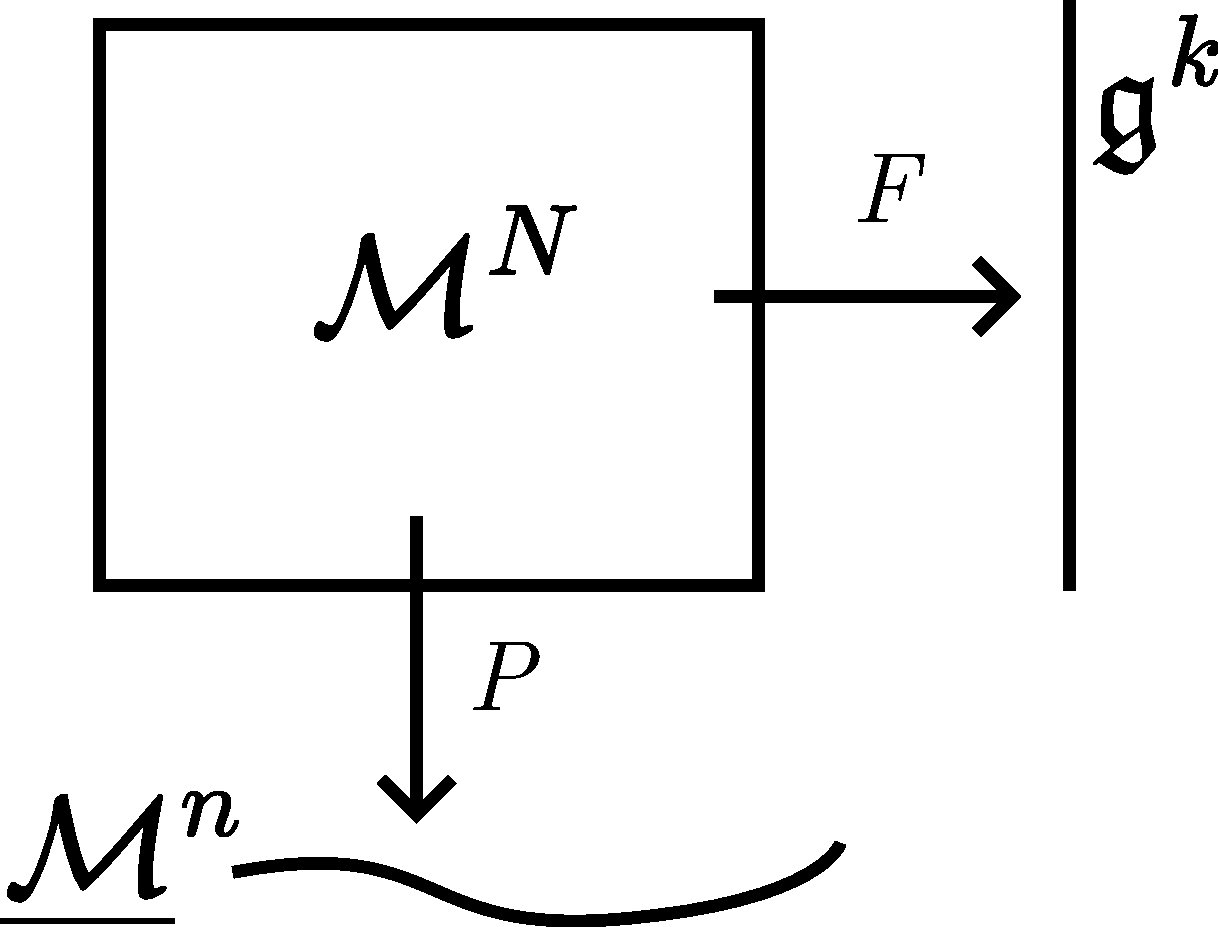
\includegraphics[width=.3\textwidth]{Drawings/Draw_2.pdf}\\
	où $\underline{\mathcal{M}}^n$ est ``espace quotient'' avec une forme volume $\underline{\omega}$.
\end{center}

\noindent \underline{Conclusion:} posant $\omega = P^* \underline{\omega}$ on a
\begin{align}
\int_\mathcal{M} \omega \quad \overset{\mathrm{gauge}\;\mathrm{fix}}{\rightsquigarrow\rightsquigarrow\rightsquigarrow}
\quad & \int_{\underline{\mathcal{M}}} \underline{\omega}\\
=& \int_\mathcal{M} (F^* \theta) \wedge (Y\lrcorner \omega)\label{GF2}\\
=& \int_\mathcal{M} (\varphi\circ F) \mathrm{det} \Big( \d (F\circ\rho)_z\Big) \omega\label{GF3}\\
=& \int_\mathcal{M} \delta_0 (F) (\mathrm{FP}) \omega \label{GF4}
\end{align}

Dans l'équation (\ref{GF2}) $\theta \in \Omega^k(\mathfrak{g})$; $\theta=\varphi\; e^1\wedge...\wedge e^k$ et $Y= Y_1 \wedge ... \wedge Y_k$ avec $Y_\alpha = \rho(e_\alpha)$. Le terme "$\mathrm{det} \Big(\d (F\circ\rho)_z\Big)$" dans (\ref{GF3}) est le déterminant de Faddeev Popov, noté FP. Enfin, le passage de (\ref{GF3}) à (\ref{GF4}) utilise le fait que $A$ peut être vue via le diagramme commutatif suivant:
$$\begin{tikzcd}
\mathfrak{g}\arrow[r, "\rho_z"]\arrow[rr,"A",bend right=30,swap] & T_x\mathcal{F}_x \arrow[r,"\d F"] & \mathfrak{g}
\end{tikzcd}$$
et pour finir, on remplace $\varphi \in \mathcal{C}^\infty_\mathrm{c}$ par $\delta_0$ sur $\mathfrak{g}$. Pour rappel, on peut voir $\delta_0$ comme limite (au sens des distrib') mais sinon, aussi via Fourrier formel:
$$\delta_0(F) = \frac{1}{(2\pi\hbar)^k}\int_{\mathfrak{g}^*} \d^4\lambda \e^{\frac{i}{\hbar}\langle\lambda,F\rangle}$$
où $\lambda \in \mathfrak{g}^*$ est un multiplicateur de Lagrange. De même FP $= \mathrm{det} \; A$ où $A=\d (F)\circ \rho$.\\

\underline{Remarque}: On a un petit problème avec FP qui n'est pas local en l'espace-temps (i.e. si on change $\mathcal M$ par $\Omega^1(\mathbb M)$, par exemple, $\mathrm{det}(A)_{z\in\Omega^1(\mathbb M)}$ ne se calcul pas à partir de la forme locale de $z$)...
\subsection{Un peu de super-calcul}
Soit:
\begin{itemize}
\item $V$ un espace vectoriel de dimension $k$;
\item $\ppi(V^*\oplus V)$ le foncteur de super-parité;
\item $\mathcal{C}^\infty\big(\ppi(V^*\oplus V)\big) = \Lambda^0(V^*\oplus V)^*$ où $\Lambda^0$ est l'algèbre extérieure;
\item $(e_1, ..., e_k)$ une base de $V$, $(e^1, ..., e^k)$ sa base duale (et on les combinera pour les bases des produits tensoriels);
\item $A\in \mathrm{End}(V)\approx V\otimes V^*$ que l'on décompose en $A=A^i_{\;j}e^j\otimes e_i$
\end{itemize}
\underline{Propriété:}
$$
I:= \int_{\ppi(V^*\oplus V)}\D c^k \D \Bar c_k ... \D c^1 \D \Bar c_1 \quad \e^{\frac i \hbar \langle \Bar c, A c \rangle}
= \left(\frac{i}{\hbar}\right)^k \mathrm{det} \; A
$$
Preuve:
\begin{align*}
\langle \bar c, A c \rangle &= \bar c_\alpha A^\alpha_{\;\beta} c^\beta &
c &\in \mathcal{C}^\infty(\ppi V^*) &
\e^{\frac i \hbar \langle\bar c, A c\rangle} &= \sum_{p=0}^\infty \frac{1}{p!}\left(\frac{i}{\hbar}\langle\bar c, Ac\rangle\right)^p\\
A &= A^\alpha_{\;\beta} e^\beta\otimes e_\alpha&
\bar c &\in \mathcal{C}^\infty(\ppi V)&
&=\sum_{p=0}^k \frac{1}{p!}\left(\frac{i}{\hbar}\langle\bar c, Ac\rangle\right)^p
\end{align*}
où les termes de degrés $>k$ disparaissent car dans l'algèbre extérieure.
\begin{align*}
I &= \int_{\ppi(V*\oplus V)} (\D c\D \bar c)^k \left(\frac i \hbar \right)^k \frac{\langle\bar c,Ac\rangle^k}{k!}&&\\
&= \left( \frac i \hbar \right)^k \frac 1 {k!} \dr{}{c^k}\dr{}{\bar c_k}...\dr{}{c^1}\dr{}{\bar c_1} \langle\bar c, Ac\rangle^k &
\mathrm{car}\;\mathrm{integrale} & \; \mathrm{de}\;\mathrm{Berezin}\\
\langle\bar c, Ac\rangle^k &= (\bar c_1 A^1+ ... + \bar c_k A^k)^k & A^\alpha &= A^\alpha_{\;\beta} c^\beta\\
&= \sum_{\alpha_1, ... \alpha_k} \sum_{\beta_1, ...\beta_k} (\bar c_{\alpha_1} A^{\alpha_1}_{\;\beta_1}c^{\beta_1})...(\bar c_{\alpha_k} A^{\alpha_k}_{\;\beta_k}c^{\beta_k})&
\langle\bar c, Ac\rangle &= \bar c_\alpha A^\alpha\\
&= \sum_{\alpha_i, \beta_i} A^{\alpha_1}_{\;\beta_1}...A^{\alpha_k}_{\;\beta_k} \times (\bar c_{\alpha_1} c^{\beta_1})...(\bar c_{\alpha_k} c^{\beta_k})
& \mathrm{les}\; (\bar c_\alpha c^\beta)\;\mathrm{commutent}&\;\mathrm{entre}\;\mathrm{eux}\\
&= k! \sum_{\beta_i} A^{1}_{\;\beta_1}...A^{k}_{\;\beta_k} \times (\bar c_{1} c^{\beta_1})...(\bar c_{k} c^{\beta_k})\\
&= k! \mathrm{det}(A)\times (\bar c_{1} c^{1})...(\bar c_{k} c^{k})& \Box
\end{align*}
\underline{Conclusion:}
$$\boxed{\boxed{
\int_{\underline{\mathcal M}} \underline \omega = \int_\mathcal M \int_{\mathfrak g^*} \d^k\lambda \left(\frac i \hbar \right)^k \int_{\ppi(\mathfrak g \oplus \mathfrak g^*)} (\D c\D\bar c)^k \e^{\frac i\hbar \Big( \langle \lambda, F\rangle+\langle\bar c, \d(F\circ \varphi) c\rangle \Big)} \omega
}}$$
Et ce qui nous intéresse est:
$$\omega := \e^{\frac\hbar i S(x)} \mathcal{O}(x) \d^N x \quad \quad \mathcal{C}\in\mathcal{C}^\infty(\mathcal{M})$$
où $\mathcal{O}$ est invariante par la jauge $\mathfrak{g}$, i.e. c'est une observable physique.

$$\boxed{\boxed{
\int_\mathcal M \e^{\frac i\hbar S} \mathcal{O} \d^N x := \frac{``\mathrm{Vol}(G)"}{(2\pi\hbar)^k}\left(\frac\hbar i\right)^k \int_\mathcal M \int_\mathfrak g \int_{\ppi(\mathfrak g^*\oplus\mathfrak g)} \d^Nx\d^k\lambda(\D c\D\bar c)^k \e^{\frac i\hbar S_{\mathrm{FP}}(x,\lambda,c,\bar c)}\mathcal{O}(x)
}}$$
où:
$$\boxed{
S_\mathrm{SP}(x,\lambda,c,\bar c):= S(x)+ \langle\lambda,F(x)\rangle + \langle\bar c, \d(F\circ \rho)_x c\rangle
}$$
\underline{Remarque}:

Ici, on a supposé que $\langle\lambda, F(x)\rangle$ ``passe une seule fois dans l'orbite". On peut généraliser à un passage à $n<\infty$ simplement en normalisant par $\frac1n$.\\\\
\underline{Interprétation:} Hessienne de $S_\mathrm{FP}$ vs celle de $S$.
$$S(x) = \underset{\mathrm{quadratic}}{Q(x)}+ \underset{\mathrm{interactions}}{\tilde S_\mathrm{int}(x)}$$
$\int \d x \e^{\frac i\hbar S_\mathrm{int}}$ n'a généralement pas de sens, mais $\int d x \e^{\frac i\hbar Q}$ (par exemple si $Q\geq 0$ mais en fait, en général il suffit qu'il soit non-dégénéré). Si $Q$ est inversible, on appel $Q^{-1}$ son ``propagateur". Le problème est qu'en théorie de jauge, $Q$ n'est pas inversible à cause de non énorme noyau. En coordonnées locales sur $\mathcal M\times\mathfrak g\times\ppi(\mathfrak g^*\oplus\mathfrak g)$:
$$\dr S{z^i}=0\quad\quad(\mathrm{symetrie}\;\mathrm{de}\;\mathrm{jauge})$$
$$\boxed{\d S_{x_0}=0}$$
i.e. $x_0$ point critique de l'action (i.e. solution d'E.L.) notons $x_0\approx(x_0,\lambda_0,c_0,\bar c_0)$ pour aller plus vite.
$$\partial^2 S_{\mathrm{F}.\mathrm{P}.}(x_0) =
\begin{matrix} & \partial_y \qquad\partial_z \qquad\partial_\lambda \quad\qquad\partial_c \qquad\partial_{\bar c}\quad\\ 
	\begin{matrix} \partial_y \\\partial_z\\\partial_\lambda\\\partial_c\\\partial_{\bar c}\end{matrix} &\left(\begin{matrix}\color{teal}\boxed{\begin{matrix}\color{red}\boxed{\begin{matrix}
	\frac{\partial^2 S}{\partial y^i \partial y^j} & 0\\
	0 & 0
\end{matrix}} & \begin{matrix}
	? \\ \frac{\partial F^\alpha}{\partial z^i}
\end{matrix}\\
\quad\quad ? \quad \quad\frac{\partial F^\alpha}{\partial z^j} & 0\end{matrix}} & \cdot\cdot\cdot\\
\cdot\cdot\cdot & \color{blue}\boxed{\begin{matrix}
0 & - ^t\d F\circ\rho\\ \d F\circ\rho & 0
\end{matrix}}\end{matrix}\right)\end{matrix}$$
Où: $\color{red}\Box=\partial^2 S_{x_0}$, \color{teal}$\Box$ est inversible\color{black},
et \color{blue} $\Box$ aussi \color{black}.\\
Remarque générale sur la notion de super-matrice: \color{teal} paire
\color{black} et \color{blue} impaire\color{black}.
$$\left(\begin{matrix}
	\color{teal}\boxed{\color{black}M_{00}} & M_{01}\\
	M_{10} & \color{blue}\boxed{\color{black}M_{11}}
\end{matrix}\right)$$
$M_{00}$ et $M_{11}$ sont à coefficients paires (Bosons) et $M_{01}$ et $M_{10}$ impaires (Fermions). 
\begin{align*}
^\mathcal{S}\mathrm{det} :&= ``\mathrm{super}\;\mathrm{determiant}"\\
:&=\frac{\mathrm{det}\left(M_{00}-M_{01}M_{11}^{\;-1}M_{10}\right)}{\mathrm{det}\;M_{11}}
\end{align*}
et $M$ inversible ssi $^\mathcal{S}\mathrm{det}\;M \ne 0$.\\L'idée derrière la construction de $^\mathcal{S}\mathrm{det}$ est que $\mathrm{det}(AB)=\mathrm{det}(A)\times\mathrm{det}(B)$ d'où: $$^\mathcal{S}\mathrm{det} \left(\begin{matrix}
M_{00}&0\\0&M_{11}
\end{matrix}\right) = \frac{\mathrm{det}\; M_{00}}{\mathrm{det}\; M_{11}}$$
\underline{Lemme:} (proof as exo)
$$\left(\begin{matrix}
M_{00} & M_{01}\\
M_{10} & M_{11}
\end{matrix}\right)
\overset{\exists X}=
\left(\begin{matrix}
M_{00}-M_{01}M_{11}^{\;-1}M_{10} & 0\\
0 & M_{11}
\end{matrix}\right)
\times
\mathlarger{\mathlarger{\Bigg(}}\left(\begin{matrix}
1 & 0\\ X & 1
\end{matrix}\right)
\mathrm{ou}
\left(\begin{matrix}
1 & X\\ 0 & 1
\end{matrix}\right)\mathlarger{\mathlarger{\Bigg)}}
$$
$\left(\partial^2S(x_0,0,c,\bar c)\right)^{-1}$ est ``l'énorme" propagateur dont on utilise des blocs.

\subsection{Application à Yang-Mills}
$$S_\mathrm{YM}= \frac{-1}4 \int_\mathbb{M}\mathrm{tr}(F\wedge*F)\quad\quad\quad A\mapsto A+\epsilon\d_A\alpha + o(\epsilon)$$
$$F: \quad \alpha \in \mathcal{C}^\infty(\mathbb{M},\mathfrak{g}) \quad \overset\rho\longrightarrow\quad  \overset{\d_A\alpha = \d\alpha+[A,\alpha]}{\Omega^1(\mathbb{M},\mathfrak{g})} \quad \underset{\mathrm{Lorentz}}{\overset{\d F}\longrightarrow} \quad \d(*\d_A\alpha)\in \mathcal{C}^\infty(\mathbb{M},\mathfrak{g})$$

$$\color{red}\boxed{\color{black}
S_\mathrm{FP}(A,\lambda,c,\bar c) = S_\mathrm{YM}(A)+ \int_\mathbb{M}\d^4x \lambda(x) \d(*A) + \int_\mathbb{M}\d^4 \bar c(x) \d(*\d_A\alpha) c(x)
\color{red}}\color{black}$$
Avec $(k_{\alpha\beta})$ la métrique de $\mathfrak{su}(p)$ et
$$F=\d A + \frac12[A\wedge A]= \d A + A\wedge A$$
on a:
\begin{align*}
S_\mathrm{YM} =& \int k_{\alpha\beta} (\partial_\mu A^\alpha_{\;\nu} - \partial_\nu A^\alpha_{\;\mu})(\partial^\mu A^{\beta\nu} - \partial^\nu A^{\beta\mu}) && (\mathrm{Maxwell})\\
&+A\cdot A\cdot\partial A + A\cdot A\cdot A&&(\mathrm{Perturbations})\\
&+\lambda\d(*A) + \underset{= \bar c \;\Box c}{\bar c\d(*\d c)} + \bar c\d(*A c) &&(\mathrm{Fantomes})
\end{align*}
On peut alors avoir: $\to \partial^2S(\rho, c) \to (\partial^2S)^{-1}(\rho,c)$
$$(\partial^2S)^{-1} = \left(\begin{matrix}
	\boxed{\begin{matrix}
	\frac{\eta^{-1}}{|\xi|^2} - \frac{\xi^\dagger \xi}{|\xi|^4}& \frac{\xi}{|\xi|^2}\\
	\frac{^t\xi}{|\xi|^2} & 0
	\end{matrix}} & \cdot\cdot\cdot\\ \cdot\cdot\cdot & \boxed{\begin{matrix}
		0 & \frac{1}{|\xi|^2}\\
		\frac{-1}{|\xi|^2} & 0
	\end{matrix}}
\end{matrix}\right)$$
où la première matrice par bloc est le propagateur.\newpage
\noindent Notons également que cela se traduit par un changement de règles de Feynman:\\

\begin{minipage}{.1\textwidth}
	\!\!\!\!\!\!\!\!\!\!\!\!\!\!\!\!\!\!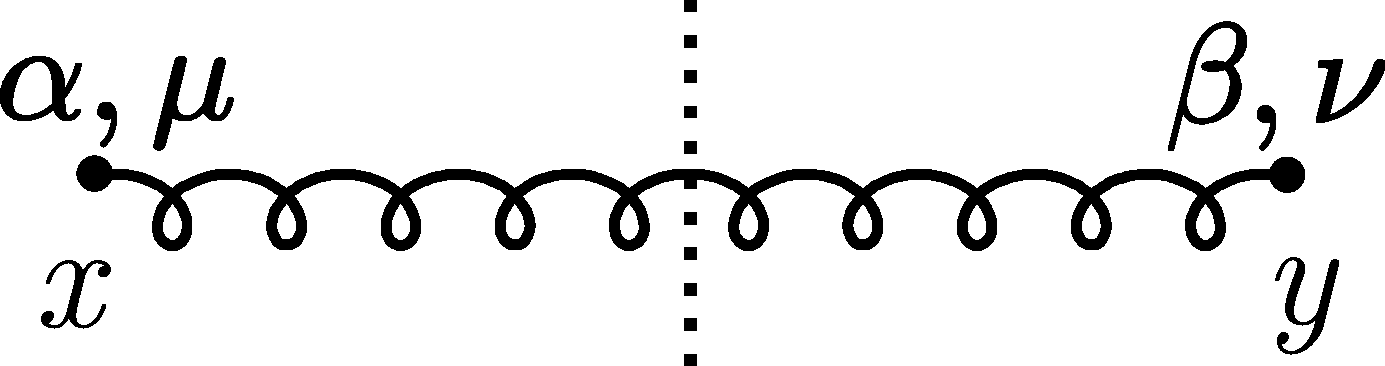
\includegraphics[width=2\textwidth]{Drawings/Draw_6.pdf}
\end{minipage}
\begin{minipage}{.9\textwidth}
	$$\!\!\!\!= \langle A^\alpha_\mu(x) A_\nu^\beta (y)\rangle  = \left(\frac{\int \D A e^{\frac{i}{\hbar}(\cdot\cdot\cdot)}A^\alpha_\mu(x)A_\nu^\beta(y)}{\int \D A e^{\frac{i}{\hbar}(\cdot\cdot\cdot)}}\right) \longrightarrow  \int \frac{\d^4k}{(2\pi)^k}e^{-ik(x-y)}\frac{i \delta_{\alpha\beta}\eta_{\mu\nu}}{k^2 \pm i\epsilon}$$
\end{minipage}

\begin{minipage}{.1\textwidth}
	\!\!\!\!\!\!\!\!\!\!\!\!\!\!\!\!\!\!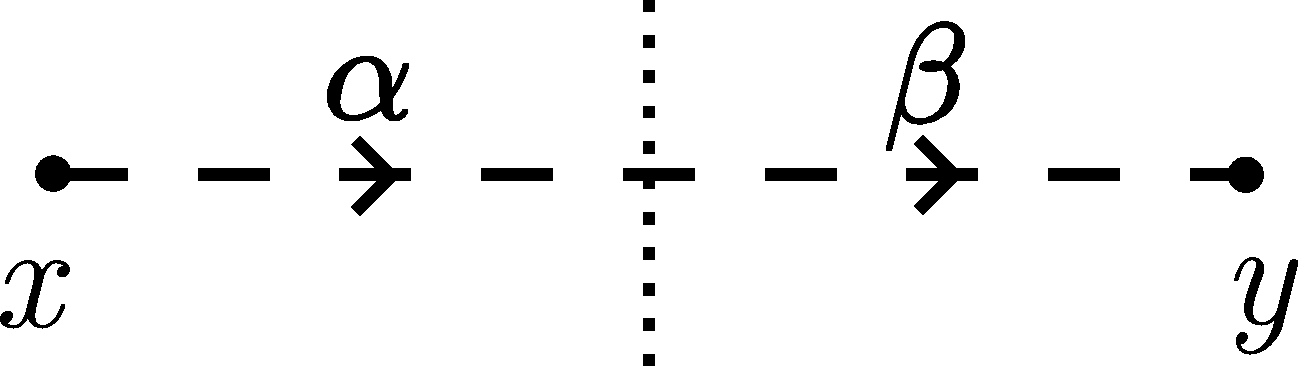
\includegraphics[width=2\textwidth]{Drawings/Draw_3.pdf}
\end{minipage}
\begin{minipage}{.6\textwidth}
	$$= \quad \langle c^\alpha(x) \bar{c}_\beta (y)\rangle \quad = \quad \int \frac{\d^4k}{(2\pi)^k}e^{-ik(x-y)}\frac{i \delta_{\alpha\beta}}{k^2 \pm i\epsilon}$$
\end{minipage}\\ \\

\noindent\underline{Interactions:}\\

\begin{minipage}{.2\textwidth}
	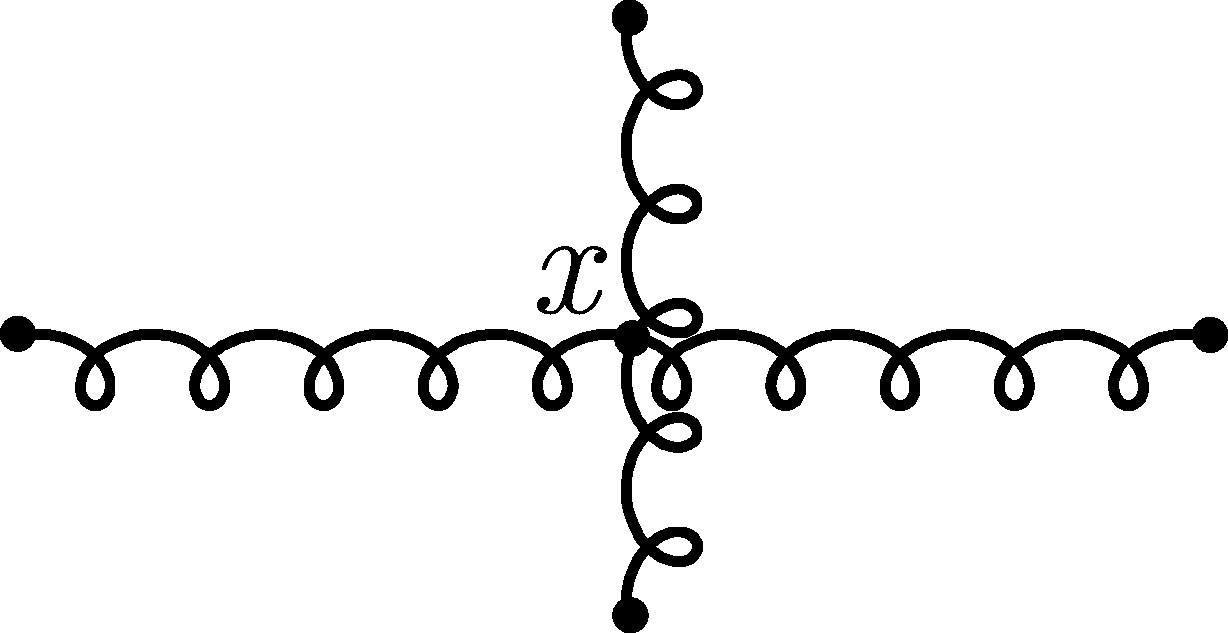
\includegraphics[width=\textwidth]{Drawings/Draw_7.pdf}
\end{minipage}
\begin{minipage}{.3\textwidth}
	$\Big([A,A]\;[A,A]\Big)(x)$
\end{minipage}

\begin{minipage}{.2\textwidth}
	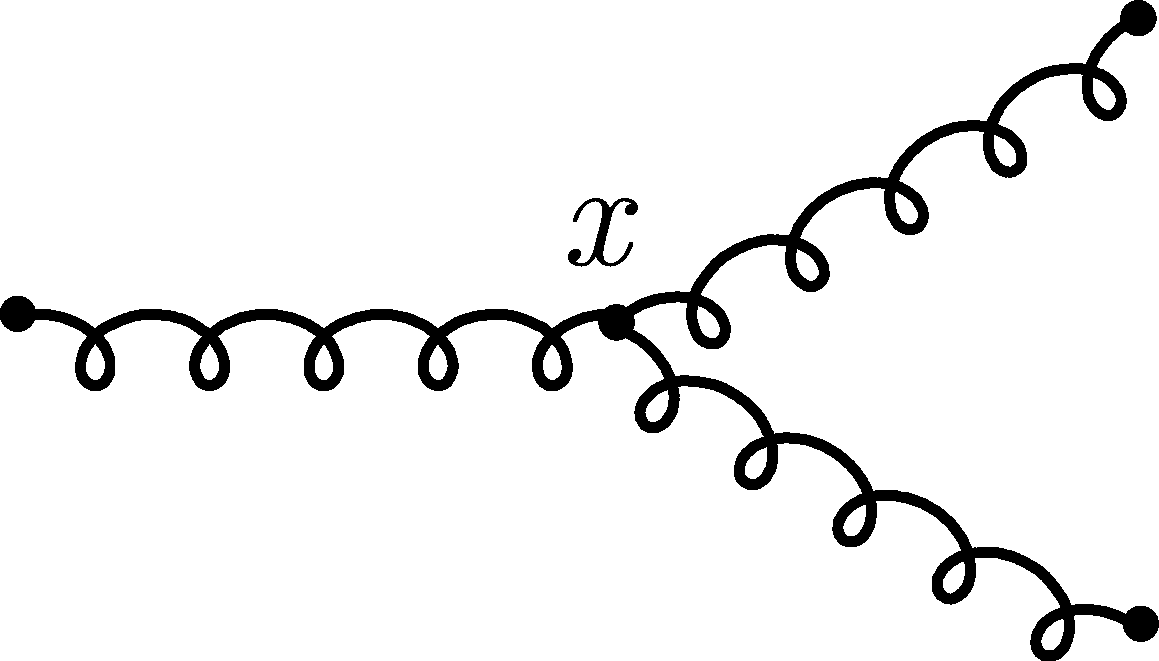
\includegraphics[width=\textwidth]{Drawings/Draw_8.pdf}
\end{minipage}
\begin{minipage}{.3\textwidth}
	$[A,A] \d A$
\end{minipage}

\begin{minipage}{.2\textwidth}
	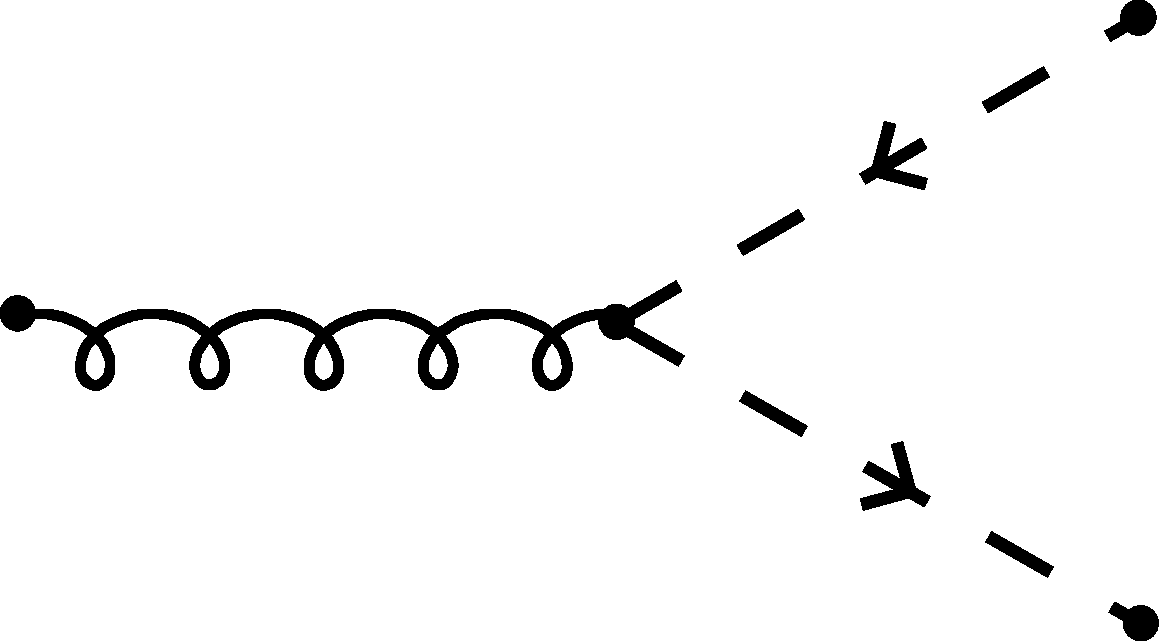
\includegraphics[width=\textwidth]{Drawings/Draw_0.pdf}
\end{minipage}
\begin{minipage}{.3\textwidth}
	$\bar c \d (*A c)$
\end{minipage}


\section{Gestion des Symétries: BRST, BV}
\subsection{Cohomologie fantôme}
\noindent Il reste à vérifier que:
\begin{itemize}
\item la théorie est bien invariante de jauge (\color{Green}\checkmark\color{black} par construction)
\item les fantômes $c$ et anti-fantômes $\bar c$ sont in-observables. (Méthode calculatoire: t'Hofft \& Veltman.) Nous allons le montrer par la méthode BRST (Becchi, Rouet, Stora \& Tyutin).
\end{itemize}
\underline{Observation:}\\
Notons que $\langle\lambda,F(x)\rangle + \langle\bar c, \d(F\circ\rho)c\rangle = \lambda_\alpha F^\alpha+\bar c_\alpha(\d F\circ\rho)^\alpha_{\;\beta} c^\beta$\\
Notons les constante de structures sur $\mathfrak{g}$ par $f^\alpha_{\beta\gamma}$ pour éviter les conflits de notations avec les fantômes.
$$\boxed{
Q:=\frac12 f^\gamma_{\alpha\beta} c^\alpha c^\beta\dr{}{c^\gamma} - c^\alpha\rho^i(e_\alpha)\dr{}{x^i}+\lambda_\alpha\dr{}{\bar c_\alpha}
}$$
agit sur $\mathcal{C}^\infty\Big(\underset x {\mathcal M}\times \underset \lambda {\mathfrak g} \times \underset{(c,\bar c)} {\ppi(\mathfrak g^*\oplus\mathfrak g})\Big) $.\\

\noindent\underline{Lemme:}\\
Soit $\psi = \bar c F(x)$:
\begin{enumerate}
\item $Q\psi = \bar c_\alpha (c^\beta \rho^i(e_\beta) \dr{F^\alpha}{x^i} + \lambda_\alpha F^\alpha = \langle\lambda,F\rangle+\bar c_\alpha (\d F\circ\rho)^\alpha_\beta$.\\
Bref, $S_\mathrm{FP}$ est une dérivée totale par cet opérateur compliqué.
\item $Q(S_0) = - c^\alpha\rho^i(e_\alpha)\dr S{x^i} = 0$ ssi $S_0$ invariante de jauge.
\item $Q^2 = 0$
\end{enumerate}
\underline{Conclusion:}
\begin{itemize}
\item et donc... $S_\mathrm{FP}:= S_0 + Q\psi$, mais ça c'est une conséquence triviale des prop ci-dessus.
\item $QS_\mathrm{FP} = Q(S_0+Q\langle\bar c, F\rangle) = QS_0 + Q^2\langle\bar c,F\rangle = 0$
\item Les ``Observables" sont donc les quantités annulées par $Q$ quotientées par l'invariance de jauge c'est à dire son image. i.e. $\mathrm{ker}\,Q/\mathrm{Im}\,Q$ i.e. une classe de cohomologie. C'est en fait la cohomologie des représentations d'algèbres de Lie.
\end{itemize}
\underline{Remarque:}\\
Pour prouver $Q^2 = 0$ le prof à fait un énorme super-calcul ultralong, ça utilisait du jaccobi et tout et tout... J'ai eu trop la flemme de noter.

Si pour l'instant on a vu $Q$ comme un opérateur, on peut également remarquer que c'est un champ de (super)-vecteurs: $Q = v^i(z,\theta)\dr{}{z^i} + v^a(z,\theta)\dr{}{\theta^a}$ avec $z=(x,\lambda)$ et $\theta = \langle c,\bar c\rangle$. Dès lors, on peut calculer sa divergence vis à vis de $\d z$ et $\D\theta$ (on utilise la notation $|v|$ pour désigner le degrés de parité de $v$):
\begin{align*}
\mathrm{div}\; Q :=& \dr{v^i}{z^i}-(-1)^{|v|}\dr{v^a}{\theta^a}\\
=& -\dr{}{c^a}\left(\frac12 f^c_{ab} c^ac^b\right)+\dr{}{x^i}(\theta^a\rho^i_a) - \dr{}{\bar c_a}\lambda_a\\
=& \frac{-1}2 \left(f^c_{ab}c^b-f^c_{ac} c^a\right)+ \theta^a\dr{\rho^i_a}{x^i}\\
=& -f^c_{cb}+\theta^a\dr{\rho^i_a}{x^i}
\end{align*}
$$\mathrm{div}\;Q = 0 \quad \iff \quad \left\{\begin{matrix} f^c_{cb}=0 & \iff & \mathfrak{g} \; \mathrm{unimodulaire} &(\mathrm{i}.\e.\; \mathrm{l}'\mathrm{action}\;\mathrm{adjointe}\\
\dr{\rho^i_a}{x^i}=0 &&&\quad \mathrm{preserve}\;\mathrm{les}\;\mathrm{volumes})
\end{matrix}\right.$$
\underline{Remarque:} du coup, cette propriété ne s'applique pas dans le cas conforme.\\

\noindent\underline{Justification de la définition:} (de la super-divergence)
$$\int\int \d z\D\theta \Big((\mathrm{div}\,Q) +Qf\Big)=0\quad \quad \quad \mathrm{si}\; f\;\mathrm{ou}\; v^i \in \mathcal{C}^\infty\Big(\mathcal M\times\mathfrak g^*\times\ppi(\mathfrak g^*\oplus\mathfrak g)\Big)$$
\underline{Corollaire:} \quad \quad div $Q=0 \quad\implies \quad \int ... Qf = 0$
\begin{align*}
(\mathrm{div}\;Q)f + Qf &= \left(\dr{v^i}{x^i}-(-1)^{|v|}\dr{v^a}{\theta^a}\right) f + v^i\dr f{x^i} + v^a\dr f {\bar c^a}\\
&=\dr{(v^if)}{x^i} - (-1)^{|v|}\dr{(v^af)}{\theta^a}
\end{align*}
en fait, $-Q$ définit une différentielle de Chevalley-Eilenberg.\\

\noindent\underline{Définition:} \quad $\d_\mathrm{CE}: \Lambda^\bullet\mathfrak g^* \longrightarrow \Lambda^\bullet\mathfrak{g}^*$
\begin{enumerate}
\item linéaire
\item anti-dérivation: $\forall\alpha\in\Lambda^p\mathfrak{g}^*,\forall\beta\in\Lambda^q\mathfrak{g}^*\quad\d_\mathrm{CE}(\alpha\wedge\beta) = (\d_\mathrm{CE}\alpha)\wedge\beta + (-1)^{|\beta|}\alpha\wedge\d_\mathrm{CE}\beta$
\item action: $\forall\alpha\in\mathfrak{g}^*=\Lambda^1\mathfrak{g}^* \quad \d_\mathrm{CE}\alpha\in\Lambda^2\mathfrak{g}^*$ et $\forall\xi,\eta\in\mathfrak{g}\quad (\d_\mathrm{CE}\alpha)(\xi,\eta) = - \alpha([xi,\eta])$
\end{enumerate}

\noindent\underline{Motivation:}\\
Soit $G$ un groupe de Lie, $\mathfrak{g}$ son algèbre de Lie.
$$\begin{matrix}
\mathfrak{g} & \to & \mathfrak{X}(G)&
\quad \quad&
\alpha\in\Omega^i(G)\otimes\mathfrak{g} &\mathrm{Mauer}-\mathrm{Cartan}\\
\xi & \mapsto & [x\mapsto x\cdot\xi]&&
\alpha(x\cdot\xi)=\xi
\end{matrix}$$
$$
\d \alpha (x\cdot\xi,x\cdot\zeta) = 
-\alpha([x\cdot\xi,x\cdot\zeta]) +
\cancel{(x\cdot\xi)\lrcorner\d(\alpha(x\cdot\zeta))} -
\cancel{(x\cdot\zeta)\lrcorner\d(\alpha(x\cdot\xi))}
$$
\underline{Autre Motivation:}

$\d_\mathrm{CE}$ est le dual de $[\cdot,\cdot]$ (un co-produit quoi). Le prof est même assez convaincu que ça forme une bigèbre (voire même une algèbre de Hopf) mais bon... Faut vérifier.

\subsection{Lien avec la théorie des représentations}
\underline{Lemme:}\\
$\forall X_1,X_2,X_3 \in \mathfrak{g}\quad \forall \alpha\in \mathfrak{g}^*$
$$\d_\mathrm{CE}(\d_\mathrm{CE}\alpha)(X_1,X_2,X_3) = \alpha([[X_1,X_2],X_3]+[[X_2,X_3],X_1]+[[X_3,X_1],X_2])$$
Bref:
$$\boxed{\boxed{\mathrm{Jacobi}\quad \iff \quad \d_\mathrm{CE}^{\;\;2}=0}}$$

\noindent\underline{Représentation} de $G$ (ou $\mathfrak{g}$) vectorielle\\
Soit $V$ un espace vectoriel (muni d'une base $e_i$), $R:G\to GL(V)$ morphisme de groupes.
$$\rho : \begin{matrix}
\mathfrak{g} & \to & \mathrm{End}(V)&\\
e_a & \mapsto & \rho_a & = (\rho^i_{ja})_{ij}
\end{matrix}\quad\quad \mathrm{issue}\;\mathrm{de}\;R\quad \quad \mathrm{t}.\mathrm{q}.\quad \quad \rho[e_a,e_b]=[\rho_a,\rho_b]$$
\underline{Chevaley-Eilenberg:} (cas de la théorie des rep') $\quad \d_\mathrm{CE}: \Lambda^\bullet\mathfrak g^*\otimes V \longrightarrow\Lambda^\bullet\mathfrak g^*\otimes V$
\begin{enumerate}
\item linéaire
\item Leibneitz
\item $\forall\alpha\in\mathfrak{g}^*\otimes V\;\forall\xi,\zeta\in\mathfrak{g}$
\end{enumerate}
$$\boxed{(\d_\mathrm{CE}\alpha)(\xi,\zeta) = \rho(\xi)(\alpha,(\zeta))-\rho(\zeta)(\alpha,(\xi)) - \alpha([\xi,\zeta])}\quad \in V$$
et si $V=\mathbb{R}$, on récupère le cas vu précédemment. On comprend que (dans le cas physique) $\rho_a(x) = \rho^i_{ja}x^j\dr{}{x^i}$ dans:
$$-\d_\mathrm{CE} \quad=\quad \frac12 f^c_{ab}c^ac^b\dr{}{c^c} - c^a\rho^i_{ja}x^j\dr{}{x^i} \quad=\quad Q$$
où $Q$ agit sur $\mathcal{C}^\infty\Big(\ppi(\underset x{\mathfrak{g}}\oplus \underset c V)\Big)$\\
\underline{Exo:} Vérifier que $Q=-\d_\mathrm{CE}$\\

\noindent\underline{Prop:}
\begin{align*}
\d_\mathrm{CE}^{\;\;2} \alpha (X,Y,Z) =& \quad\, \Big([\rho X,\rho Y] - \rho[X,Y]\Big)\alpha(Z)\\
&+ \Big([\rho Y,\rho Z] - \rho[Y,Z]\Big)\alpha(X)\\
&+ \Big([\rho Z,\rho X] - \rho[Z,X]\Big)\alpha(Y)\\
&+ \alpha \Big(\underset{=``\mathrm{Jacobiateur}"}{[X,Y],Z]+[[Y,Z],X]+[[Z,X],Y]}\Big)
\end{align*}
$$\d_\mathrm{CE}^{\;\;2}=0 \quad \iff \quad \begin{matrix}
\mathrm{Jacobi}\;(\mathfrak{g}-\mathrm{alg}\;\d\e\;\mathrm{Lie})\\
\rho: \;\mathrm{representation}
\end{matrix} \quad \iff \quad \mathrm{Donc}\;Q^2=0$$
\underline{Généralisation:}\\
Remplacer $GL(V)$ par $\mathrm{Diff}(\mathcal M)$ où $\mathcal{M}$ est un variété et $\rho : 
\mathrm{End}(V) \to \mathfrak{X}(\mathcal{M})$ ou $\mathfrak{g}\to \mathfrak{X}(\mathcal{M})$
$$Q = \frac12f^c_{ab}c^ac^b\dr{}{c^c} - c^a\rho^i_a\color{red}(x)\color{black}\dr{}{x^i}$$
Soit $\varphi\in\mathcal{C}^\infty(\mathcal M\times\ppi\mathfrak{g})$ et $K^c:=\frac12f^c_{ab}c^ac^b$:
\begin{align*}
Q^2(\varphi) =& \left( K^c\dr{}{c^c} - c^a\rho_a\right)\left(K^d\dr{}{c^d}-c^b\rho_b\right)\varphi\\
=& K^c\dr{c^c}K^d + \underset{\langle\mathrm{Sym}|\mathrm{AntSym}\rangle}{\cancel{K^cK^d\dr{}{c^c}\dr{}{c^d}}}\varphi - K^c\rho_c \varphi + K^cc^b\cancel{\rho_b\dr\varphi{c^c}} - c^a(\rho_aK^c)\dr\varphi{c^c} - c^aK^d\cancel{\dr{}{c^b}\rho_a}\varphi+\!\!\!\!\!\!\!\!\!\! \underset{\quad\quad =^1\!/\!_2c^ac^b[\rho_a,\rho_b]\varphi}{c^ac^b\rho_a\rho_b\varphi}\\
=&\frac12f^c_{ab}c^ac^b\dr{}{c^c}\left(\frac12f^d_{ef}\dr\varphi{c^d}\right) - \frac12c^ac^b\Big(f^c_{ab}\rho_e-[\rho_a,\rho_b]\Big)\varphi - \frac12 \rho_a f^c_{bd}c^ac^b\dr\varphi{c^c}\\
=& \frac12\Big(f^e_{ab}f^d_{ec}-\rho_cf^d_{ab} \Big)c^ac^bc^c \dr\varphi{c^d} +\frac12 c^ac^b\Big([\rho \,e_a,\rho \,e_b] - \rho [e_a,e_b] \Big)\varphi
\end{align*}

Or $f^e_{ab}f^d_{ec}c^ac^bc^c=0 \iff$ Jacobi et le second terme est équivalent au fait que $\rho$ soit un morphisme d'alg de Lie. Ainsi, si $\rho_cf^d_{ab}=0$ (le prof dit que ``normalement ce terme est null car $f^c_{ab}$ est constant" mais j'avoue que j'ai pas compris pourquoi...)
$$Q^2=0 \quad \iff\quad \mathrm{Lie}\;\mathrm{Alg}\;\&\;\mathrm{Representation}$$
\underline{Extension:}
à $Q\in\mathfrak X(\mathcal{M}\times\ppi\mathfrak g)$ soit au cas où $f^c_{ab}\in\mathcal{C}^\infty(\mathcal M)$ i.e. non-constant. Alors $Q^2=0$ n'équivaut plus à Jacobi et rep, mais
$$\Big(f^e_{ab}f^d_{ec}-\rho_cf^d_{ab} \Big)c^ac^bc^c=0 \quad\quad\wedge\quad\quad \mathrm{rep}$$
c'est à dire: Algebr\color{red}oïde \color{black} de Lie et représentation.

\subsection{Algébroïdes \& Groupoïdes de Lie}
\underline{Définition:} Algébroïde de Lie
\begin{itemize}
\item Une \underline{variété} (``base") $\mathcal M$
\item Un \underline{fibré} vectoriel $E\to\mathcal{M}$
\item Un \underline{crochet} sur $\Gamma(\mathcal{M},E)$ noté $[\cdot,\cdot]$
\item Une \underline{encre} $\rho:\Gamma(\mathcal{M},E)\to\mathfrak{X}(\mathcal M)$ telle que\\
\color{white}$\bullet\bullet\color{black}\bullet\;\Big(\Gamma(\mathcal M, E), \; [\cdot,\cdot]\Big)\;$\color{black} est une algèbre de Lie \\
\color{white}$\bullet\bullet\color{black}\bullet\;\;\forall\varphi\in\mathcal{C}^\infty(\mathcal{M}),\forall X,Y\in\Gamma(\mathcal{M},E) \quad [X,\varphi Y] = \varphi [X,Y] + \Big(\rho(X)\cdot\varphi\Big) Y\;$\color{black}
\end{itemize}
Remarque:
$$[X,\varphi Y] \quad=\quad \underset{\in\mathbb{R}}\varphi \underset{\in E}{[X,Y]} + \Big(\underset{\in T\mathcal{M}}{\rho(X})\cdot\varphi\Big) \underset{\in E}Y \quad=\quad \varphi [X,Y] + \rho(X)\lrcorner\d\varphi Y \quad=\quad\varphi [X,Y] + \d\varphi(\rho X) Y$$
\underline{Propriété:}
$\rho$ induit un morphisme d'algèbres de Lie:
$$\Gamma(\mathcal{M},E)\quad \longrightarrow\quad\mathfrak{X}(\mathcal{M})=\Gamma(\mathcal{M},T\mathcal{M})$$
$$\rho\Big([X,Y]_E\Big) \quad = \quad \Big[\rho(X),\rho(Y)\Big]_{T\mathcal{M}\;=\;[\cdot,\cdot]_\mathrm{Lie}}$$
Preuve:\\
On considère $\varphi\in\mathcal{C}^\infty(\mathcal{M})$ et $X,Y,Z\in\Gamma(\mathcal{M},E)$; on applique Jacobi sur $(X,Y,\varphi Z)$ puis on conclu avec un calcul peu palpitant que j'ai eu la flemme de noter.\\

\noindent\underline{Exemples:}
\begin{enumerate}
\item $\mathcal{M}=\{*\}$; $\mathfrak{g}=\Gamma(*,\mathfrak{g})$; $\rho=0$ bref... Les algèbres de Lie sont des algébroïdes de Lie...
\item $\mathcal{M}$ variété, $E=T\mathcal{M}$, $[\cdot,\cdot]$ crochet des champs de vecteurs, $\rho:T\mathcal{M}\to T\mathcal{M}$ identité.
\item Soit $(\mathcal{M},\pi)$ variété de Poisson. (voir le travail de Jean Pradines)\\
$\pi\in\Gamma(\mathcal{M},\Lambda^2T\mathcal{M})$ qu'on écrit en coordonnées: $\pi = \frac12\pi^{ij}\partial_i\wedge\partial_j$ i.e. $\pi^{ij}+\pi{ji}=0$
$$\forall f,g\in\mathcal{C}^\infty \quad \{f,g\} := \pi^{ij}\dr f{x^i}\dr g{x^j}$$
$$0=[\pi,\pi]\in\Gamma(\mathcal{M},\Lambda^3T\mathcal{M}) \quad \mathrm{crochet}\;\d\e\;\mathrm{Schrouten}-\mathrm{Nijenhies}$$
On peut définir une algébroïde de Lie sur $T^*\mathcal{M}$, prenons $\alpha,\beta\in\Gamma( \mathcal{M},T^*\mathcal{M}) =\Omega^1(\mathcal{M)}$
$$[\alpha,\beta]=L_{\pi\alpha}\beta - L_{\pi\beta}\alpha - \d\Big(\pi(\alpha,\beta)\Big)\in\Omega^1(\mathcal{M})$$
où $\pi\alpha:=\pi^{ij}\alpha_i\partial_j$ car on peut en effet voir $\pi:T^*\mathcal{M}\to T\mathcal{M}$.\\
Soit $k$ une section de $E$ qui forme une base de $E_x$ pour tout $x\in\mathcal{M}$. Soit $(e_1,...e_k)$ un repère sur $E$, on obtient une algébroïde  avec:
$$[e_a,e_b]=f^c_{ab}(x)e_c$$
$$\rho(e_a)=\rho^i_a(x)\partial_i \quad \rho:E\to T\mathcal{M}$$
Et on prend pour $[\cdot,\cdot]_E$ le crochet de Lie, i.e. $\left(f^c_{ab}f^d_{ce}+\rho^i_a\dr{f^d_{bc}}{x^i}\right)\theta^a\theta^b\theta^c=0$\\
où $\theta^a:=e^a=(e_a)^*$ et $\theta^a\theta^b:=e^a\wedge e^b$...\\
$\rho$ induit un morphisme $\Gamma(\mathcal M, F) \to \mathfrak{X}(\mathcal M)$ ce qui est équivalent à dire que:
$$\rho^i_a\dr{\rho^j_b}{x^i}-\rho^i_b\dr{\rho^i_a}{x^i} - f^c_{ab}\rho^j_c = 0$$
\end{enumerate}
\underline{Idée:}

C'est un peu comme pour une paire $(A,\rho)$ d'une alg de Lie et sa représentation, si ce n'est que contrairement au cas de $\rho:A\to V$ on ne peut pas ``décrocher" $A$ de sa représentation car les coefficients sont non-constants et dépendent de la variété.\\

\noindent Si $\varphi = \varphi^a e_a$ et $\psi=\psi^be_b \in \Gamma(\mathcal{M},E)$
\begin{align*}
[\varphi,\psi]_E &= [\varphi^ae_a,\psi^be_b]\\
&= \varphi^a[e_a,\psi^be_b] - \d\varphi^a \Big(\rho(\psi^be_b)\Big)e_a\\
&= \varphi^a\Big(\psi^b[e_a,e_b]+\d\psi^b(e_a)e_b\Big)-\psi^b\d\varphi^a(e_b)e_a\\
&= \varphi^a\psi^b[e_a,e_b] + \varphi^a\d\psi(\rho_a)e_b - \psi^b\d\varphi^a(\rho_b)e_a\\
&=\Big(f^c_{ab}\varphi^a\psi^b + \varphi^a\rho^i_a\dr{\psi^c}{x^i} - \psi^b\rho^i_b \dr{\varphi^c}{x^i}\Big)e_c
\end{align*} 
\underline{Cas Poisson:}
\begin{align*}
\rho(\d x^i) &= \pi^{ij}\partial_i\\
[\d x^i,\d x^j] &= \d \pi^{ij} = \dr{\pi^{ij}}{x^k} \d x^k\\
\implies [\alpha,\beta]_{T^*\mathcal{M}} &= [\alpha_i \d x^i, \beta_j \d x^j]_{T^*\mathcal M}\\
&= \Big[\partial_k \pi^{ij}\alpha_i\beta_j + \pi^{ij}(\alpha_i\partial_j\beta_k - \beta_i \partial_j \alpha_k)\Big]\d x^k
\end{align*}
\underline{Lien avec les groupoïdes de Lie:}\\ \\
\underline{Définition:} Groupoide de Lie

On demande à ce que $G$ et $G^{(0)}=:\mathcal{M}$ soient des variétés. On demande également un plongement $\mathcal{C}^\infty$, tel que $G$ soit une sous-variété de $G^{(0)}$, $u: \mathcal{M}\hookrightarrow G$, et évidement on demande que les opérations de compositions soient lisses.\\


\noindent\underline{Lien avec alg de Lie:}
$$T^bG = \Big\{(\gamma,v) \in TG; \d b_\gamma(v)=0\in T_{b(v)}\mathcal{M}\Big\}\quad\subset\quad TG$$
$$u*T^bG = T^bG|_\mathcal{M} = \Big\{(x,v); x\in \mathcal{M}; v\in T_x ^b G\Big\}$$
Bref, les ``plans tangents" aux unités forment une algebroide de Lie.\\

\noindent\underline{Remarque sur le problème inverse:}

Aller d'algeboide vers groupoide n'est pas du tout aussi simple. En fait, c'est presque un problème ouvert. Il y a un théorème qui permet d'intégrer une algèbroide de Lie en un groupoide ($3^\e$ théorème de Lie, par Cartan et Edo) mais la structure de Lie est assez bouleversée donc on sait pas trop ce que c'est. La question de la structure de ces groupes a été posée par Alan Winster, (c'est une sorte de variété ultra singulière) et la réponse est en partie venue de la Physique.\\

\noindent\underline{Exemple de Groupoïde de Lie:}\\
$G$ un groupoide, $\mathfrak{g}$ son algèbre; le groupoide associé est:
$$T^*G = \mathfrak{G} \quad \mathfrak{g}^*=\mathfrak{G}^{(0)}$$
Et on a une application ``moment": $T^*G \to \mathfrak{g}^*$ qui permet bien de voir le plongement.

\subsection{Méthode BV}
\underline{Quantification BRST:}
$$\int_{\mathcal M \times \mathfrak g \times \ppi(\mathfrak g^* \oplus \mathfrak g)}\!\!\!\!\!\!\!\!\!\!\!\!\!\!\!\!\!\!\!\!\!\!\!\!\!\d x\; \d\lambda\; \D c\; \D\bar c \quad \e^{\frac i\hbar \Big(S(x)+\langle\lambda,F(x)\rangle+\langle\bar c, (\d F\circ \rho) c\rangle\Big)}$$
où $F:\mathcal{M}\to\mathfrak g$ fixe la jauge, et $\langle\lambda,F(x)\rangle+\langle\bar c, (\d F\circ \rho) c\rangle = Q\langle\bar c, F(x)\rangle$
$$Q^2 = \frac12 f^c_{ab}c^ac^b\dr{}{c^c} - c^a\rho^i_a(x) \dr{}{x^i}+\lambda_a \dr{}{\bar c_a}$$
$$Q^2 = 0 \quad \quad \wedge \quad \quad QS=0=-c^a\varphi^i\dr{}{x^i} \quad Q\mathcal{O}=0$$
\underline{Une autre méthode: BV} (Batalin Vilkovisky)
$$\mathcal N := \mathcal{M}\times\mathfrak g \times \ppi(\mathfrak g^* \oplus \mathfrak g) \quad \quad z=(x,\lambda,c,\bar c)$$
$$\rightsquigarrow \quad \ppi T^*\mathcal N = \Big\{ (z,z^\dag), \; z\in\mathcal N, \; z^\dag\in\ppi T^*_z\mathcal N\Big\}$$
$$\mathcal C^\infty (\ppi T^*_z\mathcal N) = \Lambda^0 (T_z\mathcal N) \quad \quad \quad
z^\dag = (x_i^\dag, \lambda^a_\dag, c_a^\dag, \bar c_\dag^a)$$
\underline{Remarque Historique:}

J. Zinn-Justin (des français) ont introduit le même objet, pas pour résoudre les problèmes de Jauge, mais pour la renormalisation, c.f. Weinberg, tomme II chapitre 1 \& 2.
\begin{align*}
\mathrm{Sur}\;\ppi T^*\mathcal N, \quad \omega &= \d z^\dag_n \wedge \d z^n\\
&= \d x^\dag_i\wedge \d x^i \;+\; \d \lambda^\alpha_\dag \wedge \d \lambda_a \;+\; \d c^\dag_a\wedge \d c^a \;+\; \d\bar c^a_\dag \wedge \d \bar c_a
\end{align*}
$\theta = \color{violet}z^\dag_n\color{black}\d z^n$ et $Q\in\mathfrak{X}(\mathcal{M})$. En voyant $Q$ comme un champ de vecteur $Q\lrcorner \theta\in\mathcal{C}^\infty(\ppi T^*\mathcal{M})$ ce qui n'est pas sans rappeler Noether symplectique.
\begin{align*}
Q\lrcorner\theta =& \frac12 f^c_{ab}c^ac^b\color{violet}c^\dag_c &&&& \theta = p_i\d q^i\\
&-c^a\rho^i_a(x)\color{violet}x^\dag_i &&&& \{\theta(X),H\}=0\\
&+\lambda^a\color{violet}\bar c^a_\dag &&&& \color{violet}\mathrm{Variables}\;``\mathrm{exotiques}"\color{black}
\end{align*}
$$S_\mathrm{BV}(z,z^\dag) \quad = \quad S_0(x) \quad + \quad \underset{\quad =:S_1}{Q\lrcorner\theta}$$
Notons que, en soit, BV n'a pas de gauge-fixing, mais on peut toujours le rajouter comme dans BRST.
$$S_0(x) \quad \longrightarrow \quad S_0 + \underset{\mathrm{Sym}}Q\underset{\mathrm{Gauge}\;\mathrm{Fix}}{\langle\bar c, F\rangle}$$

\noindent Comment retrouver la symétrie?
$$\frac{S_\mathrm{BV}\overset\leftarrow\partial}{\partial z_n^\dag}\;\frac{\overset\to\partial S_\mathrm{BV}}{\partial z^n} \quad = \quad 0$$
Qui est une sorte de crochet de Poisson (c'est un crochet de BV) $=\frac12 \{S_\mathrm{BV},S_\mathrm{BV}\}$
\begin{align*}
\{\varphi,\psi\} :=& \frac{\varphi\overset\leftarrow\partial}{\partial z_n^\dag}\;\frac{\overset\to\partial \psi}{\partial z^n} - (-1)^{(1+|\varphi|)(1+|\psi|)}\frac{\psi\overset\leftarrow\partial}{\partial z_n^\dag}\;\frac{\overset\to\partial \varphi}{\partial z^n}\\
\frac{S_\mathrm{BV}\overset\leftarrow\partial}{\partial z_n^\dag}\;\frac{\overset\to\partial S_\mathrm{BV}}{\partial z^n} =& 
(-c^a\varphi^i_a) \left(\dr{S_0}{x^i} - c^a\dr\varphi{x^i} \color{violet}x^\dag_j\color{black}\right) + \underset{\dr{}\lambda}0\times (c_a^\dag)\\
&+\frac12 f^c_{ab}c^ac^b\left(f^d_{cb}c^b\color{violet}c^\dag_d\color{black}-\rho^i_c\color{violet}x^\dag_i\color{black}\right) + \lambda^a \times 0\\
=& \underset{\mathrm{Sym}\;\mathrm{Jauge}}{-c^a\rho^i_a \dr{S_0}{x^i}} + \underset{\mathrm{repr}}{\left(\frac12 f^c_{ab}c^ac^b\rho_c - c^ac^b\rho^i_a \dr{\rho_b}{x^i}\right)}\color{violet}x^\dag\color{black} + \underset{\mathrm{Jacobi}}{\frac12 f^c_{ab}f^d_{cb} c^ac^bc^c} \color{violet}c_d^\dag\\
S_\mathrm{BV} =& S_0 + S_1\\
S_1 =& z_n^\dag Q z^n = c_a^\dag Q c^a+x_i^\dag Qx^i+\bar c^a_\dag Q \bar c_a\\
=& \frac12 c_c^\dag f^c_{ab}c^ac^b - x_i^\dag c^a\rho^i_a+\bar c_\dag^a\lambda_a\\
\{S_\mathrm{BV},S_\mathrm{BV}\} =& \{S_0,S_0\} + 2\{S_0,S_1\} + \{S_1,S_1\}
\end{align*}
\begin{itemize}
\item $\{S_0,S_0\}$ toujours nul car variété classique donc crochet de Poisson classique.
\item $\{S_0,S_1\}$ symétrie de Jauge.
\item $\{S_1,S_1\} \quad \rightsquigarrow\quad Q^2=0$
\end{itemize}

Quand à la gestion de la fixation de Jauge, on l'obtient par la restriction à une Lagrangienne (une surface Lagrangienne, i.e. une surface de dimension moitié sur laquelle s'annule la forme symplectique, et évidement, il y a tout un travail pour montrer qu'une telle physique est indépendante de ce choix, pour ne pas casser l'invariance de Jauge).
$$\mathrm{Jauge}: \quad L \quad \subset \quad \ppi T^* \mathcal{N}$$
\underline{Remarque:} On appelle l'équation $\{S,S\}=0$ l'équation maitresse classique.\\

Le problème, c'est qu'il existe des cas où $Q^2\ne0$ et donc $\{S_1,S_1\}\ne 0$. On suppose que $\{S_1,S1\}$ s'annule sur les points critiques c'est à dire $\underset{(\mathrm{E}.\mathrm{L}.)}{\d S_0=0}$. On parle de symétrie ``On Shell". D'où on a bien $Q^2=0$ mais seulement là où $\d S=0$. (Notons que cette affirmation nécessite également quelques hypothèses de régularité et de d'autres choses, qu'on va mettre sous le tapis). Cela a également pour conséquence que pour tout $\xi,\zeta\in\mathfrak{g}$ l'action de $\rho$ sur les champs n'est plus compatible avec le crochet de Lie i.e. $[\rho \xi, \rho \zeta]\ne \rho[\xi,\zeta]$ sauf bien sûr, sur les points où $\d S_0 = 0$.\\

\noindent \underline{Lemme:} (modulo les mêmes hypothèses) 
$$\exists E = \frac12 E^{ij}(\xi,\zeta) \partial_i\wedge\partial_j \quad \mathrm{t}.\mathrm{q}.\quad  [\rho \xi, \rho \zeta] = \rho[\xi,\zeta] + E^{ij}(\xi,\zeta) \dr S{x^i} \dr{}{x^j}$$

Cet écart à une symétrie complète n'est pas traitable avec BRST, mais ça se joue ``à pas grand chose" ($E$) et BV permet de gérer ça. Et l'idée est assez simple: on rajoute des termes:
$$\rightsquigarrow S = S_0 + S_1 + S_2\quad\quad\quad S_2 = \pm \frac12 x_i^\dag x_j^\dag E^{ij}_{\;\;ab}c^ac^b$$
$\{S,S\}$ est alors sans termes de degrés 1 i.e. homogène de degrés 2 en les antichamps.

\subsection{Retour sur la Fixation de Jauge dans le cas BV}
\underline{Avec BRST:} \quad $S_0 + Q\psi$ où $\psi:=\bar c_a F^a(x)$ fixe la jauge.\\\\
\underline{Avec BV:}
$$\int_\mathcal{N} \e^{\frac i\hbar S_\mathrm{BV}} \quad\quad\rightsquigarrow\quad\quad
\int_{L\subset \ppi T^*\mathcal{N}} \e^{\frac i\hbar S_\mathrm{BV}} \quad L\; \mathrm{sous}-\mathrm{varr}\;\mathrm{Lagrangienne}$$
\begin{align*}
S_\mathrm{BV} &= S_0 + S_1 (+S_2 +...)\\
&= S_0 + Q \lrcorner Q\\
L &= \left\{\Big(z^n, z_n^\dag= \dr\psi{z^n}\Big) \quad z \in \mathcal{N} \right\} && \subset \ppi T^*\mathcal{N}\\
Q &= z_n^\dag\d z^n &&\in \Omega^1(\ppi T^*\mathcal N)
\end{align*}
\underline{Sous-varr Lagrangienne:} (Mécanique)
\begin{itemize}
\item Soit $(Y,\omega)$ une varr symplectique; $n:= \mathrm{dim} Y$.\\
Une \emph{sous-variété Lagrangienne} $L$ est une sous-varr de dim $^n\!/\!_2$ et telle que $\omega|_L=0$
\item Localement: $Y + T^* X$, et $\omega = \d p_i \wedge \d q^i$
$$L = \left\{\Big(x^i,\dr S{x^i}\Big)\quad x\in X\right\} \quad \mathrm{pour}\;\mathrm{un}\;\mathrm{certain}\; S:X\to\mathbb{R}$$
(modulo les singularités, évidement, cf la lagrangienne pour une courbe de la forme $\color{red}\cdot\color{black}\!\!\! \subset$ dans le cours d'analyse micro-locale I...)
$$S_1 = z_n^\dag Q z^n \quad\quad S_1|_L = \dr \psi{z^n} Q z^n = \bar c_a \dr{E^a}{x^i} Q x^i + F^aQ \bar c_a$$
\end{itemize}
\underline{Remarque:}

Il existe un théorème (via un calcul diff extérieur, en dim infinie, et une sorte de thm de Stockes) qui donne une contrainte sur BV pour s'assurer de l'indépendance de $\int_L \e{^i\!/\!_\hbar S_\mathrm{BV}}$ par des déformations homologiques de $L$; permettant ainsi de récupérer l'invariance de jauge (qu'on aurait pu pensé perdue dans la fixation de jauge).\\

\noindent\underline{Autre remarque:}\\
On peut construire une mesure ``Berezinienne" sur $\d z^n$ sur $L \subset \ppi T^*\mathcal{N}$.\\ 
Bere $\approx \dr{}{z^1}\wedge...\dr{}{z^p}\lrcorner \mathrm{forme}$
$$\overset{\mathrm{pair}}{z^n} \quad \longrightarrow\quad \overset{\mathrm{impair}}{z^\dag_n}\quad \quad \quad \d z^\dag_n\approx\dr{}{z_n^\dag}\approx\d z^n
\quad \quad \quad (\mathrm{tres}\;\mathrm{vaguement})$$

C'est le tour de magie qui assure que l'on a une bonne mesure sur $L$ indépendante des coordonnées, via de la dualité bien trouvée. cf le livre de Pavel-Nev pour la construction.

\subsection{Toute petite aparté sur la quantification}
\underline{Exemple:} Kontsevitch (1997) formule de quantification par déformation d'une variété de Poisson.\\

\noindent\underline{Le problème:}
$F \in \mathcal{C}^\infty(T^*\mathcal M) \rightsquigarrow \Hat F$ opérateur sur $\mathcal{H}\approx L^2(X)$\\
Approche par déformation: 
$$\Big( \mathcal{C}^\infty(T^*X), \{\cdot,\cdot\}\Big) \quad \overset{\mathrm{quantification}}\longrightarrow (\mathcal{A},[\cdot,\cdot])$$

$\mathcal{A}$ une algèbre d'opérateurs auto-adjoints. Notons que si ça marche pour les variétés, c'est vite assez limité. On généralise donc un chouille en cherchant à créer un $*$-produit $(fg)\mapsto f * g$ (qui sera donc \#, le produit de Moyal dans le cas pseudo-diff) tel que:
$$f*g \quad\quad = \quad\quad f \cdot g \quad+\quad \hbar \{f,g\} \quad+ o(\hbar^2)$$
puis on se pose le même problème, mais sur une variété de Poisson:
$$\Big(\mathcal M, \underset{=\pi}{\{\cdot,\cdot\}}\Big) \quad \quad \quad fg \quad \mapsto \quad f*g = f\cdot g + \hbar \{f,g\} + ...$$
1999 Fattaneo \& Felder formulent une interprétation de la formule de Konsevitch.

\section{Modèle Poisson-$\Sigma$}
\subsection{Contexte}
On se donne $(\mathcal{M},\{\cdot,\cdot\}) = (\mathcal{M},\pi)$ une variété de Poisson. 
\begin{center}
	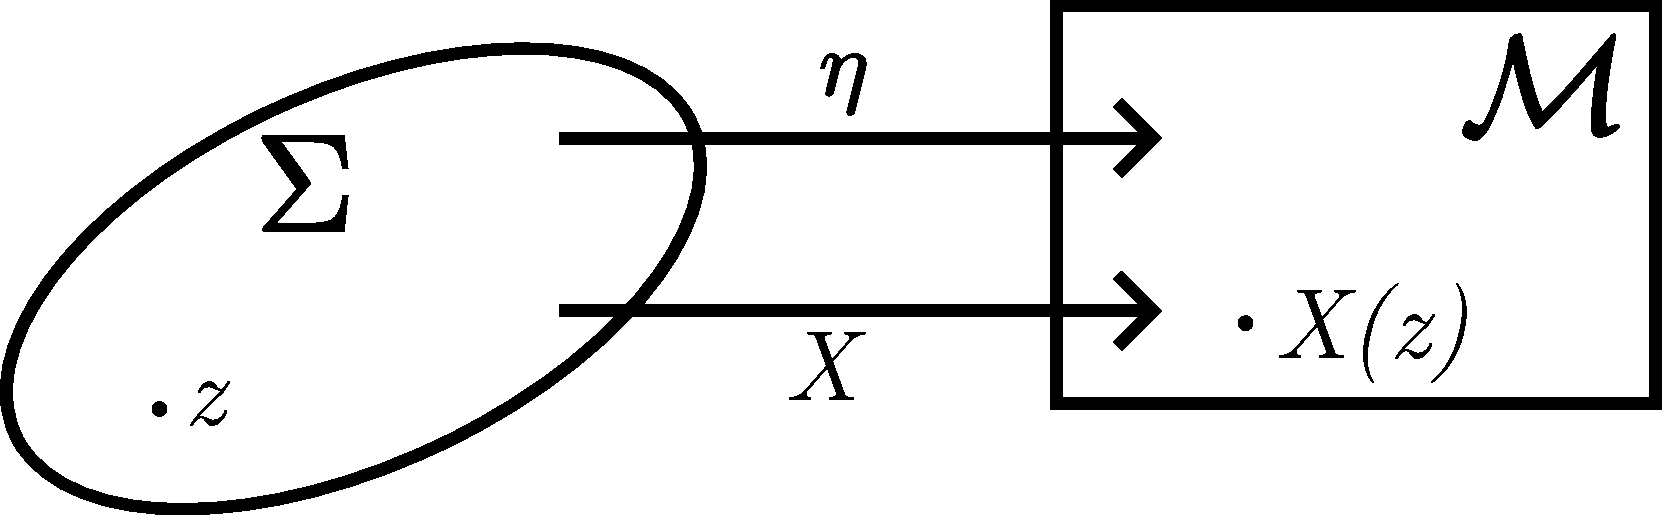
\includegraphics[width=.5\textwidth]{Drawings/Draw_4.pdf}
\end{center}
$$X \in \mathcal{C}^\infty (\Sigma,\mathcal M)\quad\quad\quad \eta \in\Omega^1(\Sigma)\otimes_X X^*T^*\mathcal{M}$$
$$\mathrm{en}\; z \in \Sigma, \quad \eta_z \in T^*_z Z \otimes T^*_{X(z)}\mathcal{M}$$
Notons que si $\Sigma$ est un tube, on obtient les théories des cordes.\\ \\
On se munit de coordonnés $x^i$ sur $\mathcal{M}$; $\eta = \eta_i \d x^i:= \eta_i\otimes \d x^i$ où $\eta_i \in \Omega^1(D)$.
$$S(X,\eta) = \int_{\Sigma^2} \eta_i \wedge \d X^i + \frac12 \pi^{ij} (x) \eta_i\wedge \eta_j $$
\underline{Remarque:} cette action est topologique.

\begin{center}\begin{minipage}{.2\textwidth}\begin{center}
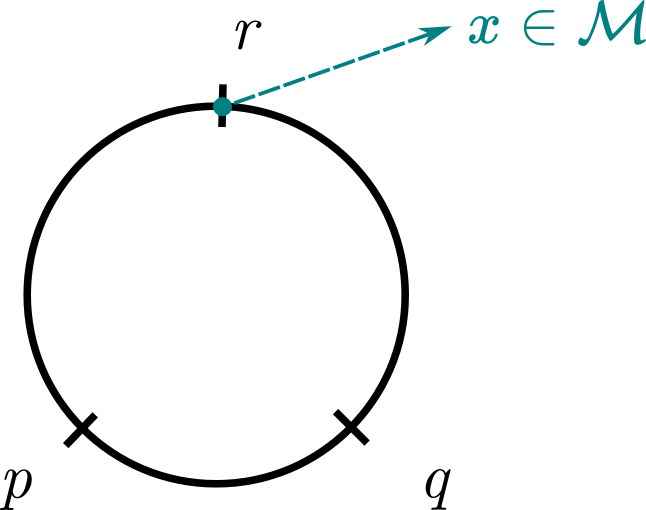
\includegraphics[width=.9\textwidth]{Drawings/Draw_5.png}
\end{center}
\end{minipage}\begin{minipage}{.4\textwidth}
$$\int_{(X,\eta)} \D X \D \eta \e^{\frac i\hbar S(X,\eta)} \underset{=(f*g)(x)}{f(X(p))g(X(q))}$$
\end{minipage}\end{center}
$X(r)=x$, mais aussi $p,q,r \in \partial \Sigma$ et $f,g\in\mathcal C^\infty (\mathcal{M})$. Calculons E.L.
$$\left\{\begin{matrix}
\d X^i \;+\; \pi^{ij} (x)\eta_j &=& 0\\
\d \eta_i + \frac12 \partial_i \pi^{jk}(x) \eta_j\wedge\eta_k \!\!\! &=& 0
\end{matrix}\right.$$
\underline{Remarque:} Les variations sont toutes à support compact, d'où l'absence de termes de bord.
\subsection{Symétrie de Jauge}
\quad Pour $b\in \mathcal C^\infty(\Sigma, X^*T^*\mathcal M)$ où $X^*T^*\mathcal M$ est le fibré de base $\Sigma$ dont la fibre en $z$ est $T^*_{X(z)}\mathcal{M}$, i.e. $b=b_i \d x^i$ avec $b_i \in\mathcal{C}^\infty(\Sigma)$. Notons que c'est une symétrie modulo un terme de bord.\\

\noindent\underline{Rappel:}

$(\mathcal{M},\pi)$ est une algébroide de Lie. Or, le dual d'une alg de Lie est une varr de Poisson. D'où le dual d'une varr de Poisson est aussi une algebroide de Lie. (enfin, là, ``avec les mains"). Donc $T^*\mathcal M$ algébroïde de Lie. $(X,\eta)$ est alors une 1-forme à coefficients dans une algébroïde de Lie.\\\\
\underline{L'algebroïde de Lie:}
$$\begin{matrix}
T^*\mathcal{M} &\quad \quad \quad & \mathrm{Crochet}\;\mathrm{sur}\; \Gamma(T^*\mathcal{M})\\
\downarrow\\
\mathcal{M} && \mathrm{Ancre}\;\rho: T^*\mathcal{M} \quad \longrightarrow \quad T\mathcal{M}
\end{matrix}$$
$$[X,fY] = f[X,Y] + (\rho(X)\lrcorner \d F)Y \quad\quad\quad X,Y\in\Gamma(T^*\mathcal{M})$$
$$[\d x^i, \d x^j] \quad=\quad \d \pi^{ij} \quad=\quad \partial_k \pi^{ij} \d x^k
\quad\quad\quad\quad\quad\rho(\d x^i) \quad=\quad \pi^{ij}\partial_j\quad\quad\quad\quad\quad
\d X \quad=\quad \rho(\eta)$$
$$\d\eta_i + \frac12[\d x^j, \d x^k] \eta_j\wedge\eta_k \quad = \quad 0 \quad\quad\quad /\!/\mathrm{Mauer}-\mathrm{Cartan}: \; \d A^a + \frac12 f^a_{bc}A^bA^c = 0$$
\underline{Interprétation:} la connexion a ne courbure nulle dans l'espace des phases.
$$\delta_b X \quad=\quad \rho_X (b) \quad\quad\quad\quad\quad \delta_b \eta \quad = \quad \d^\nabla b$$

$\d^\nabla$, la ``différentielle covariante"  construite via les $\partial_i \pi^{jk}$ qui jouent le rôles des constantes de structure en théorie de Lie.\\ \\
Dans une illustration dimension-finie:
$$Q_{T^*\mathcal{M}} = -\frac12 \partial_k \pi^{ij}(x) \alpha_i\alpha_j \dr{}{\alpha_k} + \pi^{ij} \alpha_i \dr{}{x^j}$$

$(x^i,\alpha_j)$ coordonnées sur $T^*\mathcal{M}$ de sorte que $\alpha = \alpha_i \d x^i$. On voit alors $T^*\mathcal{M}$ est vue comme algebroïde de Lie, et on a recréé un ``Chevaley-Eilenberg" pour $T^*\mathcal{M}$: ${Q_{T^*\mathcal{M}}}^2 = 0$.\\

\noindent\underline{Cas dimension infinie:} (toujours Poisson-$\Sigma$)

On a une représentation de $\mathcal{C}^\infty(\Sigma, T^*\mathcal{M})$ sur $\eta \in \Omega^1(\Sigma)\otimes_X X^*T^*\mathcal M$ avec $X:\Sigma\to\mathcal{M}$ et $\beta \in \mathcal{C}^\infty(\Sigma)\otimes_X X^*T^*\mathcal{M} = \Gamma(\Sigma,X^*T^*\mathcal{M})$.
$$Q_{X^*T^*\mathcal M} = -\frac12 \partial_k \pi^{ij}(X) \beta_i\beta_j\dr{}{\beta_k} + \pi^{ij}(X) \beta_i \dr{}{x_j} + (\d \beta_i + \partial_i \pi^{jk}(X)\eta_j \beta_k) \dr{}{\eta_i}$$
et: \quad ${Q_{X^*T^*\mathcal{M}}}^2 \ne 0$\quad\quad (d'où l'échec d'une approche BRST)
$$=\left(-\frac12 \partial_i \partial_l \pi^{jk}(X) \beta_j\beta_k(\d X^l + \pi^{lm} \eta_m)\right)\dr{}{\eta_i} \quad\quad\quad\quad\quad\quad\quad\quad$$

Mais on remarque dans l'expression de ${Q_{X^*T^*\mathcal{M}}}^2$ le terme $\d X^l + \pi^{lm} \eta_m$ qui n'est autre qu'une des deux équations d'E.L. donc on a quand même ${Q_{X^*T^*\mathcal{M}}}^2=0$ on shell.\\
On rappelle les conditions de bord sur $(X,\eta)$ à savoir: $\langle\eta,\d X\rangle\Big|_{\partial\Sigma} = 0$, puis on pose:

$$S_\mathrm{BV} \quad := S_0 \;+\; S_1\;+\;S_2$$

$$\underline{\mathrm{Rappel}\;\mathrm{super}\;\mathrm{important}:}\quad \quad \boxed{\boxed{\;\,[\pi,\pi]^{ijk} = 2 \left(\pi^{li}\partial_l \pi^{jk} + \pi^{lj}\partial_l\pi^{ki} + \pi^{lk}\partial_l \pi^{ij}\right)\;\Bigg.}}\quad\quad\quad\quad\quad\quad\quad\quad$$
\begin{align*}
S_1 :=& \int_\Sigma - \frac12 \beta^i_\dag \Big( \partial_i \pi^{jk}(X)\beta_j \beta_k\Big) + X_j^\dag \pi^{ij}(X)\beta_i + \eta^i_\dag \Big( \d\beta_i + \partial_i \pi^{jk}(X)\eta_j\beta_k\Big)\\
S_2 :=& \int_\Sigma \frac14 \eta^i_\dag \eta^j_\dag \partial_i\partial_j\pi^{kl}\beta_k\beta_l\\
\{S_1,S_0\} =& \pm \int_\Sigma \frac14 \underset{=0}{[\pi,\pi]^{ijk}}\beta_k \eta_i\wedge\eta_j + \d(X^i\d \beta_i)\\
=& \pm \int_\Sigma \d(X^i\d \beta_i)\\
=& 0\\
\{S_1,S_1\} =& ?
\end{align*}
$$\delta_b \eta_i = \d b_i + \partial_i \pi^{jk}(X)\eta_j b_k \quad\quad\quad\quad b: \Sigma\to X^*T^*\mathcal{M}$$
\underline{Remarque:} Il est également nécessaire que l'égalité suivante soit vérifiée, mais malheureusement, le prof ne sais plus d'où ça sort...
$$\int_{\partial\Sigma} X^i\d \beta_i \quad = \quad 0$$
$$X^i\Big(\d b_i + \partial_i \pi^{jk}(X)\eta_jb_k\Big)\bigg|_{\partial\Sigma} = 0$$
\begin{align*}
\{S_1,S_2\} =& \int_\Sigma -\frac12 \eta^i_\dag \partial_i\partial_l \pi^{jk}(X) \beta_j\beta_k \Big(\underset{\mathrm{E}.\mathrm{L}.}{\d X^l + \pi^{lm}\eta_m}\Big)\\\\
&\quad \left.\begin{array}{l}
+ \beta^k_\dag \partial_k (\frac14 [\pi,\pi]^{jlm} \beta_j\beta_l\beta_m)\\\\
+ X^\dag_j (-\frac14 [\pi,\pi]^{jkl}\beta_k\beta_l)\\\\
+ \frac14\eta^i_\dag \partial_i \left([\pi,\pi]^{jkm}\right)\eta_j\beta_k\beta_m
\end{array}\right\} = 0 \; \mathrm{par}\;\mathrm{la}\;\mathrm{structure}\;\mathrm{Poisson}\; [\pi,\pi]=0\\\\
\{S_2,S_0\} =& \frac{S_2\overset\leftarrow\partial}{\partial z_n^\dag}\;\frac{\overset\to\partial S_0}{\partial z^n} + \frac{S_0\overset\leftarrow\partial}{\partial z_n^\dag}\;\frac{\overset\to\partial S_2}{\partial z^n}\\
=& \int_\Sigma \left(\frac12 \eta^i_\dag \partial_i\partial_j \pi^{kl} \beta_k\beta_l\right)\!\!\!\!\!\!\!\!\!\!\!\!\!\!\!\!\!\! \underset{\quad\quad\quad=\d X^j + \pi^{jk} \eta_k}{\dr{S_0}{X^j}}
\end{align*}
Où l'on remarque que, comme on est en dimension infinie, $\dr{S_0}{X^j}$ est un opérateur d'E.L.\\ On conclu:
$$\{S_1,S_1\}\;+\;2\{S_0,S_2\} \quad = \quad 0$$
On montre également que:
$$\{S_1,S_2\}\quad = \quad\frac14 \eta^l_\dag\eta^m_\dag\partial_l\partial_m \left([\pi,\pi]^{ijk}\beta_i\beta_j\beta_k\right) \quad = \quad 0$$
Et que (mais flemme) $\{S_2,S_2\} = 0$ ce qui permet de conclure que :
$$\boxed{\boxed{\{S_\mathrm{BV},S_\mathrm{BV}\} \; = \; 0}}$$
Dès lors: $\quad \d_\mathrm{CE} \rightsquigarrow Q \rightsquigarrow \{S_\mathrm{BV}, \cdot\}$\\
``Jaccobi": $\{\varphi,\{\psi, \chi\}\} = \{\{\varphi,\psi\},\chi\} + (-1)^{(1+|\varphi|)(1+|\psi|)}\{\psi,\{\varphi,\chi\}\}$\\
Conséquence: $\mathrm{Ad}_{S_\mathrm{BV}} := \{S_\mathrm{BV},\cdot\} \implies {\mathrm{Ad}_{S_\mathrm{BV}}}^2 = 0$

Bref, on est revenu à de la théorie connue. Notant $\{\varphi, \psi\chi\} = \pm \{\varphi,\psi\}\chi \pm \psi\{\varphi,\chi\}$. Petite remarque, tout comme en théorie des opérades, on a en fait, deux degrés qui cohabitent. Le degrès de forme $\Omega^\bullet(\Sigma)$ (0,1 et 2) et un degrès plus algébrique (-2,-1, 0 et 1) que l'on récapitule dans le tableau ci-dessous, notamment en précisant les quels sont {\color{blue} commutatifs} et {\color{red}anti-commutatifs}:
\begin{center}
	\begin{tabular}{|c|ccc|}
		\hline
		& 0 & 1 & 2\\ \hline
		-2 & && $\color{blue}\beta^i_\dagger$\\
		-1 & & $\color{blue}\eta^\dagger_i$ & $\color{red}X^\dagger_i$\\
		0 & $\color{blue}X^i$ & $\color{red}\eta_i$ & \\
		1 & $\color{red}\beta_i$ & & \\\hline
	\end{tabular}
\end{center}

\noindent Bref, notre espace des phases est:
$$\Sigma\times\mathcal{C}^1(\Sigma,\mathcal{M}) \oplus \Gamma(\Sigma,X^*T\mathcal{M})\times \mathcal{C}^1(\Sigma,X^*T^*\mathcal{M})$$
évidement, de dimension infinie.\\

\noindent\underline{Fixation de Jauge:}\\
Choix de 
$$\underset{z=(x,c,\bar c, \lambda)}{\Psi : \mathcal{N}} \longrightarrow \underset{\;\;:=\ppi\mathbb{R}}{``\mathbb{R}^{0|1}"}$$
$$L := \left\{\Big(z,\dr\Psi z\Big), \; z\in\mathcal{N}\right\} \quad \subset \ppi  T^*\mathcal{N}\quad \mathrm{varr}\;\mathrm{Lagrangienne} $$
\begin{center}
	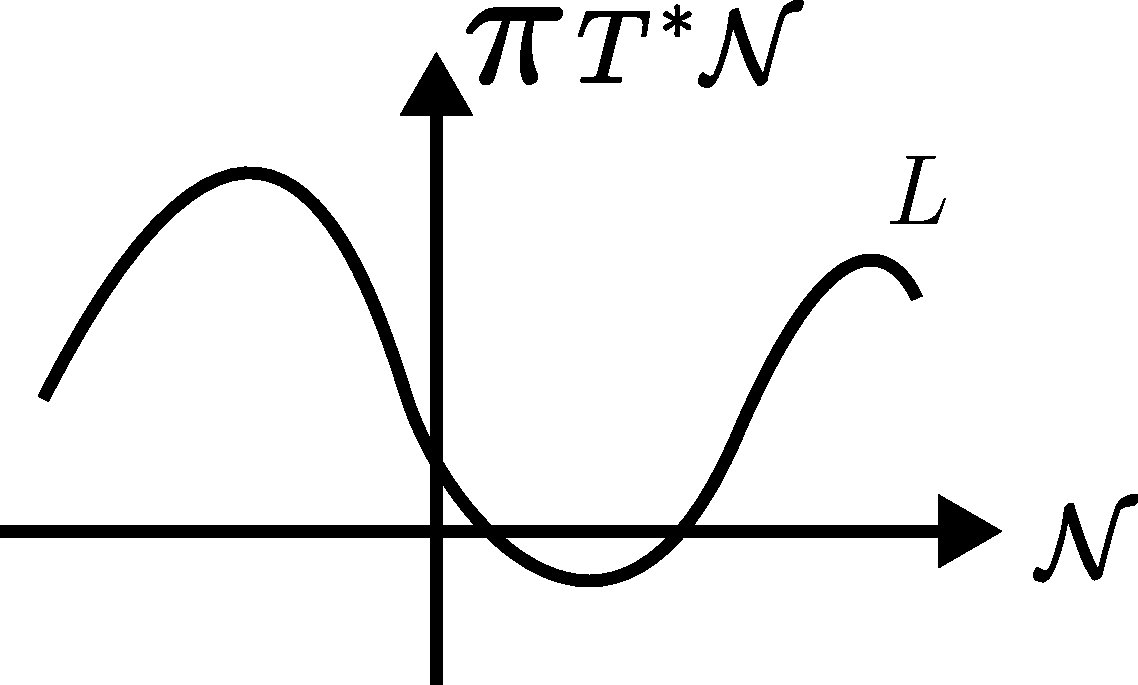
\includegraphics[width=.3\textwidth]{Drawings/Draw_9.pdf}
\end{center}

Le problème est que $\mathrm{rg}\; \partial^2 S_\mathrm{BV} \approx \mathrm{dim}\mathcal{N}$, (approximativement bien sûr, car une Lagrangienne peut avoir des points singuliers, mais en gros, c'est ça). Bref, $\partial^2S_\mathrm{BV}|_L$ est inversible, ce qui est cool, car alors $\exists G$ et on peut faire du Feynman.\\

\noindent\underline{Invariance par choix de Jauge:} (i.e. par choix de $L$)\\
Dans le cas dimension finie:\\

\begin{minipage}{.15\textwidth}
	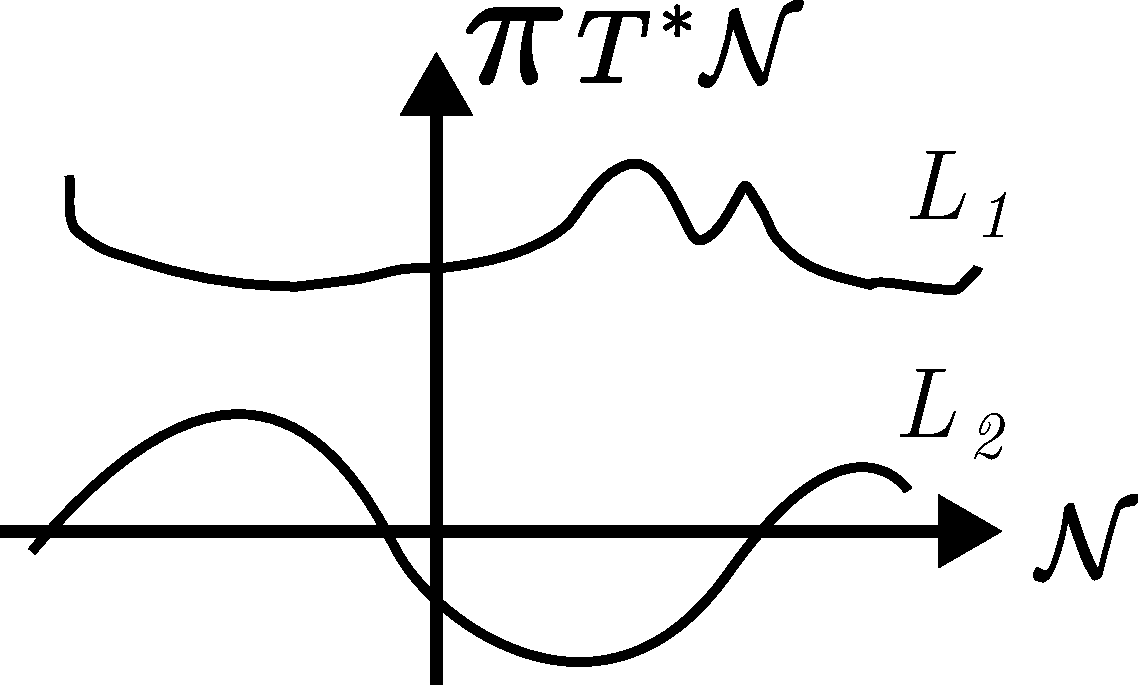
\includegraphics[width=\textwidth]{Drawings/Draw_10.pdf}
\end{minipage}
\begin{minipage}{.85\textwidth}
	$$\int_{L_1} \alpha = \int_{L_2} \alpha \quad \quad \mathrm{si}\; L_1 \sim L_2 \;\mathrm{quand}\;\mathrm{on}\;\mathrm{restreint}\;\mathrm{sur}\; \d\alpha=0$$
\end{minipage}\\

En dimension infinie, on remplace la différentielle $\d  \rightsquigarrow \Delta_\mathrm{BV} = (-1)^{|z^\dag_n|} \frac{\vec\partial}{\partial z^n}\frac{\vec\partial}{\partial z^\dag_n}$, c.f. A. Schwarz pour les détails. Considérons le cas simple suivant:
\begin{align*}
&\mathcal{N} = \mathbb{R}^n && x^i\\
&\& \; \ppi T^*\mathbb{R}^n && x_i^\dag \approx p_i
\end{align*}
$$\mathcal{C}^\infty(\ppi T^*\mathbb{R}^n) \ni X = \frac 1{k!} X^{i_1, ... i_k} \dr{}{x^{i_1}}\wedge ...\wedge \dr{}{x^{i_k}}$$
$$\dr{}{x^\dag_i} X = \d x^i \llcorner X \quad \implies\quad \dr{}{x^i} \left(\dr{}{x^\dag_i} X\right) = \dr{}{x^i}\left(\d x^i \llcorner X\right)$$
$$\d x^i \llcorner X = X^i \quad \implies \quad \Delta X = \dr{X^i}{x^i} = \mathrm{div} X = \frac{\d \Big( X^i \partial_i \lrcorner (\d x)^n\Big)}{(\d x)^n}$$
$$\Delta : \Omega^k \longrightarrow \Omega^{n-k}$$
D'où $\Delta$ : truc de dim inf ($\mathcal{N}$) $\longrightarrow$ truc de codim finie (donc c'est à peu près apréhendable).
$$\Delta^2 = 0 \quad (\mathrm{Schwarz} - \mathrm{BV})$$
\underline{Remarque de Tomas:} en vrai c'est pas trop une différentielle, mais cet objet existe en théorie de Hodge, c'est (en gros) $\d(*\d(\cdot))$ donc rien de follichon.\\

Si $\alpha$ est une fonction, $\d z$ est alors une forme de degrés moitié. Si $\Delta \alpha = 0$ et $L_1\sim L_2$ on obtient bien:
$$\int_{L_1} \alpha \d z = \int_{L_2} \alpha \d z$$ maintenant, on veut regarder si:
$$\Delta(\e^{\frac i\hbar S_\mathrm{BV}}F) \overset?= 0$$
Pour finir la construction de notre calcul diff, il ne reste plus qu'à pouvoir gérer la mesure:\\

\noindent\underline{Théorème:}
$$\Delta(\e^{\frac i\hbar S_\mathrm{BV}}) = \frac{i}{\hbar} \left(\Delta S + \frac{i}{\hbar} \{S,S\}\right) \e^{\frac i\hbar S}$$
Donc:
$$\Delta(\e^{\frac i\hbar S})=0 \quad \iff \quad \boxed{\Delta S + \frac{i}{\hbar} \{S,S\} = 0}_{\;\mathrm{equation}\;\mathrm{maitresse}\;\mathrm{quantique}}$$

Dans beaucoup de modèles, $\Delta S = \{S,S\} = 0$, du coup, c'est facile. Et c'est le cas, pour Poisson-$\Sigma$.
$$\Delta(\e^{\frac i\hbar S_\mathrm{BV}}F) = \Delta(\e^{\frac i\hbar S_\mathrm{BV}})F \pm \mathrm{cste}\underset{=0}{\{S,F\}} \e^{\frac i\hbar S_\mathrm{BV}}$$
où le crochet s'annule par invariance de jauge de $F$ i.e. indep des anti-champs.\\
\underline{Rappel de règle de calcul:} $\Delta(\varphi\psi) = \Delta\varphi \psi + (-1)^{|\varphi|}\{\varphi,\psi\} + (-1)^{|\varphi|} \varphi\Delta\psi$\\

\noindent\underline{Lemme:}
\begin{itemize}
\item $\{S,S^n\} = n S^{n-1} \{S,S\}$
\item $\Delta S^n = n S^{n-1} \Delta S + \frac{n(n-1)}2 S^{n-2}\{S,S\}$
\end{itemize}
Preuve: récurrence simultanée\\

Ceci permet de conclure qu'on peut faire Feynman sur Poisson-$\Sigma$; tout en conservant l'invariance de Jauge, et toutes les bonnes propriétés physiques.\\

\noindent\underline{Fixation de Jauge Alternative:} (chez Cattaneo \& Felder)

On fait un calcul perturbatif, $X=x+\xi$ avec $x\in\Sigma$; $\xi \in \mathbb{R}^n$ et $\eta$ ``petit". On rajoute à l'action:
$$+ S_\mathrm{gh} = \int_\Sigma \eta_i (\d\xi^i + * \d \chi^i) + \beta_i \d * \d \gamma^i$$
$\beta_i$ fantôme, $\gamma^i$ fantômes, et $\lambda^i$ multiplicateurs de Lagrange.\\
\underline{Remarque du prof:} un bon choix de Jauge, serait alors $\d(*\eta)=0$

Avec cela, Cataneo et Felder re-dérivent la formule de Kontsevitch (fort lie avec les algebroïdes de Lie). C'est également comme cela qu'ils construisent un groupoide (presque de Lie, mais singulier) qui integre tout algebroide de Lie (inspiré de la structure de Poisson de Poisson-$\Sigma$). 
\begin{align*}\underset{\mathrm{chemins}=\quad\quad\quad}P\!\!\!\!\!\!\!\!\!\!\!\!\!\!\!\!T^*\mathcal{M} =& \mathcal{C}^1([0,1], T^*\mathcal M)\\
=& \{(X,\eta), X:[0,1] \to \mathcal{M}, \eta\in\Omega^1([0,1])\otimes_X X^*T^*\mathcal{M}\}
\end{align*}
$$\delta_\beta X^i = -\pi^{ij}(X)\beta_j\quad\quad\quad \delta_\beta \eta_i = \d \beta_i + \partial_i \pi^{jk}(X) \beta_k$$
$$\mathrm{dim}\{\mathrm{orbites}\;\mathrm{dans} PT^*\mathcal{M}\;\mathrm{sous} \mathrm{l}'\mathrm{action}\;\d\e\;\mathcal{C}^\infty(T^*\mathcal{M})\}=2n=2\mathrm{dim}\mathcal{M}=\mathrm{grp}-\mathrm{oid}\;\d\e\;\mathrm{Lie}$$
\end{document}